\documentclass[journal]{IEEEtran}
\renewcommand{\rmdefault}{cmr}
\renewcommand{\sfdefault}{cmss}
\renewcommand{\ttdefault}{cmtt}
\usepackage{amsmath,amssymb,amsfonts}
\usepackage{graphicx}
\usepackage{algorithm}
\usepackage{algorithmic}

\begin{document}

\title{Industrial Adaptive Hybrid Event-Driven Spoofing Detection (IAH-EDSD) for Resource-Constrained Wireless Sensor Networks}

\author{\IEEEauthorblockN{1\textsuperscript{st} Prashanth K}
\IEEEauthorblockA{\textit{Department of Master of Computer Applications} \\
\textit{RV College of Engineering(Affiliated to VTU, Belagavi)}\\
Bengaluru, India \\
prashanthk@rvce.edu.in}
\and
\IEEEauthorblockN{2\textsuperscript{nd} Usha J}
\IEEEauthorblockA{\textit{Department of Master of Computer Applications} \\
\textit{RV College of Engineering(Affiliated to VTU, Belagavi)}\\
Bengaluru, India \\
ushaj@rvce.edu.in}
}

\markboth{IEEE Transactions on Industrial Informatics}{Karthik et al.: Industrial Adaptive Hybrid Event-Driven Spoofing Detection (IAH-EDSD)}

\maketitle

\begin{abstract}
Wireless Sensor Networks (WSNs) deployed in modern industrial telemetry, smart manufacturing, and critical infrastructure environments are severely exposed to active identity spoofing and Sybil attacks. While continuous cryptographic signature verification---such as Elliptic Curve Digital Signature Algorithm (ECDSA-P256)---provides unforgeable origin authentication, its computational overhead ($\sim 90$~mJ per verification on 16-bit MSP430-class sensor microcontrollers) rapidly depletes node batteries, creating an unsustainable security-energy trade-off. To resolve this dilemma, we present the \textbf{Industrial Adaptive Hybrid Event-Driven Spoofing Detection (IAH-EDSD)} framework, engineered to deliver the \textbf{optimal energy-security trade-off} for industrial WSNs. IAH-EDSD replaces static continuous authentication with event-driven triggers based on physical-layer Received Signal Strength Indicator (RSSI) bounds and packet rate spikes. It incorporates an adaptive multi-factor dynamic trust engine ($T = \alpha T_{\text{auth}} + \beta T_{\text{behavior}} + \gamma T_{\text{energy}}$) with real-time context-aware weight updating, an Early Warning Score (EWS) temporal convergence accumulator, and a novel \textbf{energy-adaptive detection mode switching} mechanism (FULL/LIGHT/EVENT\_ONLY) that selectively activates computational modules based on residual node battery levels. Validated through extensive discrete-event NS-3 simulations across a 401-node industrial factory floor ($1000\text{ m} \times 1000\text{ m}$) under realistic telemetry workloads ($1,120,555$ packets), IAH-EDSD selectively triggers heavy cryptographic audits on only $0.53\%$ of incoming traffic. Cryptographic validation is triggered in less than $0.53\%$ of total packet events (bypassing $99.47\%$ during steady state), ensuring minimal impact on overall energy consumption. This cuts per-packet evaluation energy consumption by $99.40\%$ (from $90.00$~mJ down to $0.540$~mJ) while maintaining $98.18\%$ spoofing detection accuracy, an exceptionally low $0.03\%$ false positive rate, and extending cluster head network operational lifetime by over $130\times$.
\end{abstract}

\begin{IEEEkeywords}
Wireless Sensor Networks (WSNs), Identity Spoofing Detection, Physical-Layer Security, Adaptive Trust Management, Resource Minimization, Industrial Internet of Things (IIoT), NS-3 Discrete-Event Simulation.
\end{IEEEkeywords}

\section{Introduction}
Wireless Sensor Networks (WSNs) form the digital backbone of the Industrial Internet of Things (IIoT), enabling continuous environmental monitoring, factory automation, process control, and predictive maintenance across smart manufacturing plants and critical infrastructure~\cite{ref_iot_survey_01, ref_wsn_ind_02}. In typical industrial deployments, hundreds of resource-constrained sensor nodes collect telemetry data (such as temperature, vibration, pressure, and flow rates) and relay packet transmissions across multi-hop clustered topologies toward a centralized Base Station (BS) or industrial edge gateway~\cite{ref_cluster_03, ref_iiot_sec_04}.

However, due to the open broadcast nature of wireless communication channels, lack of physical tamper-resistance in industrial field devices, and strict energy budgets, industrial WSNs are exceptionally vulnerable to active wireless attacks~\cite{ref_phy_sec_05, ref_wsn_threats_06}. Among these, \textbf{Identity Spoofing} and \textbf{Sybil attacks} pose severe security risks. In an identity spoofing attack, an adversary masquerades as a legitimate sensor node by forging its Media Access Control (MAC) or Network-Layer ID, injecting malicious control signals, corrupting sensor measurements, or disrupting cluster routing paths~\cite{ref_spoof_survey_07, ref_sybil_08}. In a Sybil attack, a single compromised or rogue node simultaneously claims multiple fake sensor identities, gaining disproportionate influence over cluster head election algorithms and data aggregation protocols~\cite{ref_sybil_wsn_09}.

To protect against origin spoofing, conventional network security frameworks mandate continuous public-key cryptographic signature verification---most notably using Elliptic Curve Cryptography (ECDSA NIST P-256) or HMAC authentication for every transmitted packet~\cite{ref_ecc_wsn_10, ref_crypto_cost_11}. Although continuous cryptographic authentication delivers robust security assurances against identity forgery, it incurs an unsustainable computational and energy tax on resource-constrained sensor hardware~\cite{ref_mcu_energy_12}. Experimental benchmarks on 16-bit MSP430-class sensor microcontrollers (operating at 8 MHz) demonstrate that verifying a single ECDSA-P256 digital signature consumes approximately $90.0$~mJ of electrical energy and takes upwards of $1.2$ seconds of processing time~\cite{ref_ecdsa_bench_13, ref_msp430_bench_14}. For Cluster Heads (CHs) processing thousands of telemetry packets per hour, continuous signature verification leads to rapid battery depletion, node premature failure, network partitioning, and catastrophic loss of operational monitoring capacity~\cite{ref_ch_depletion_15}.

Conversely, lightweight non-cryptographic anomaly detection schemes---such as pure Received Signal Strength Indicator (RSSI) fingerprinting or standalone machine learning (ML) classifiers---offer micro-joule operational overhead ($5$--$100\,\mu\text{J}$) but suffer from elevated False Positive Rates (FPR) under industrial radio interference, multipath fading, and dynamic shadowing effects~\cite{ref_rssi_fading_16, ref_ml_ids_17}. Pure ML models operating in static regimes fail to adapt when physical channel conditions fluctuate or when network energy levels drop, leading to either security breaches or unnecessary alarm generation~\cite{ref_adaptive_trust_18}.

To resolve this critical energy-security trade-off, this paper proposes the \textbf{Industrial Adaptive Hybrid Event-Driven Spoofing Detection (IAH-EDSD)} framework. IAH-EDSD bridges physical-layer radio propagation properties, lightweight machine learning, dynamic multi-factor trust evaluation, and conditional cryptographic verification into a multi-tier defense architecture tailored for large-scale industrial WSNs.

\subsection{Research Motivations and Key Contributions}
The primary objective of this research is to design, mathematically formulate, simulate, and validate a resource-minimized spoofing detection engine capable of maintaining near-perfect detection accuracy while cutting cryptographic energy tax by over $95\%$. The specific contributions of this work are summarized as follows:

\begin{enumerate}
    \item \textbf{Industrial Adaptive Hybrid Architecture (IAH-EDSD)}: We propose a multi-tier spoofing detection engine integrating physical-layer spatial RSSI fingerprinting, lightweight anomaly scoring, dynamic trust evaluation, and selective on-demand ECDSA-P256 signature verification.
    \item \textbf{Event-Driven Monitoring Mechanism}: We formulate an event-driven trigger function that bypasses computationally intensive security checks during normal steady-state operations and activates security audits only upon detecting packet rate spikes ($>12$~pkts/s), spatial RSSI discrepancies ($>5.0$~dBm), or unmapped node join requests.
    \item \textbf{Context-Aware Dynamic Weight Adaptation}: We formulate an adaptive multi-factor trust engine aggregating authentication trust ($T_{\text{auth}}$), behavioral spatial consistency ($T_{\text{behavior}}$), and residual energy ($T_{\text{energy}}$). Dynamic weights ($\alpha(t), \beta(t), \gamma(t)$) adjust in real time based on instantaneous network traffic spikes, battery depletion rates, and industrial radio interference.
    \item \textbf{Early Warning Score (EWS) Convergence Engine}: We formulate a temporal EWS accumulator that tracks historical suspicion event ratios, enabling rapid convergence for intermittent spoofing attacks while suppressing false alarms caused by transient shadowing noise.
    \item \textbf{Energy-Adaptive Detection Mode Switching}: We formulate a three-tier energy-adaptive detection mode selection mechanism $\mathcal{M}(E_{\text{ratio}})$ that dynamically adjusts detection complexity based on residual node energy: FULL detection ($E_{\text{ratio}} > 0.70$), LIGHT detection ($0.30 < E_{\text{ratio}} \leq 0.70$), and EVENT\_ONLY monitoring ($E_{\text{ratio}} \leq 0.30$), progressively disabling expensive ML and cryptographic modules as battery levels decline.
    \item \textbf{Large-Scale Industrial NS-3 Validation and NetAnim Trace Export}: We implement the complete IAH-EDSD framework in NS-3 discrete-event simulator across a 401-node industrial topology ($1000\text{ m} \times 1000\text{ m}$) under realistic telemetry workloads ($1,120,555$ packets). We export the complete spatial setup to NetAnim XML trace format (\texttt{iah\_edsd\_netanim.xml}) and validate that IAH-EDSD achieves a $99.40\%$ energy reduction.
\end{enumerate}

\subsection{Paper Organization}
The remainder of this paper is structured as follows. Section~\ref{sec_related_work} provides a detailed literature review and comparative taxonomy of existing spoofing detection methods. Section~\ref{sec_system_model} details the industrial network topology, microcontroller energy accounting model, radio channel propagation, and threat models. Section~\ref{sec_methodology} presents the formal mathematical formulation and algorithmic procedure of the proposed IAH-EDSD framework. Section~\ref{sec_experimental_setup} outlines the NS-3 discrete-event simulation setup, cppyy C++ bindings, machine learning training, and NetAnim integration. Section~\ref{sec_results} presents empirical benchmark results, accuracy metrics, energy savings, network lifetime extension, and comparative discussions. Section~\ref{sec_conclusion} concludes the paper and discusses future research directions.

\section{Related Work and Literature Survey}
\label{sec_related_work}

Spoofing attack detection in Wireless Sensor Networks has been widely studied across four primary paradigms: (i) Physical-Layer Radio Fingerprinting, (ii) Cryptographic Origin Authentication, (iii) Trust and Reputation Security Models, and (iv) Machine Learning Anomaly Classifiers.

\subsection{Physical-Layer Radio Fingerprinting}
Physical-layer security approaches leverage inherent physical characteristics of wireless radio propagation---such as Received Signal Strength Indicator (RSSI), Channel State Information (CSI), Phase Difference of Arrival (PDoA), and Angle of Arrival (AoA)---to authenticate node origin without relying on secret keys~\cite{ref_phy_sec_05, ref_rssi_finger_19}. 

Yang \textit{et al.}~\cite{ref_yang_rssi_20} proposed K-means clustering over RSSI spatial profiles to detect identity spoofing in IEEE 802.11 networks. Their approach demonstrated that spatial correlation between RSSI readings from different antenna receivers can effectively distinguish legitimate transmissions from spoofed signals originating from distinct spatial locations. However, their model assumed stationary radio channels without heavy industrial multipath fading.

Liu \textit{et al.}~\cite{ref_liu_csi_21} utilized fine-grained CSI amplitude and phase features from OFDM subcarriers to detect spoofing in industrial wireless networks. While CSI provides higher spatial granularity than RSSI, acquiring CSI requires specialized software-defined radio (SDR) hardware or modified Wi-Fi NIC drivers, rendering it impractical for low-cost IEEE 802.15.4 / ZigBee sensor nodes. Furthermore, environmental changes---such as moving industrial machinery or overhead cranes---cause rapid spatial decorrelation, resulting in elevated false positive rates ($>12\%$)~\cite{ref_csi_fading_22}.

\subsection{Cryptographic Origin Authentication Schemes}
Cryptographic approaches guarantee origin authenticity using symmetric MACs or asymmetric digital signatures~\cite{ref_crypto_cost_11}. Heinzelman \textit{et al.}~\cite{ref_leach_sec_23} integrated symmetric key pre-distribution into clustered WSN architectures (SecLEACH). While symmetric HMAC checks incur low computational overhead ($<10\,\mu\text{J}$), key compromise at a single sensor node exposes the entire cluster to impersonation and Sybil attacks.

To prevent master key compromise, public-key cryptographic primitives---specifically Elliptic Curve Cryptography (ECC)---have been implemented for WSNs~\cite{ref_ecc_wsn_10}. Public-key schemes like TinyECC~\cite{ref_tinyecc_24} and ECDSA NIST P-256 enable unforgeable per-packet signature generation and verification. However, performance studies by Piotrowski \textit{et al.}~\cite{ref_mcu_energy_12} and Wandeler \textit{et al.}~\cite{ref_msp430_bench_14} proved that verifying an ECDSA-P256 signature on 16-bit sensor microcontrollers (e.g., TI MSP430 or Atmel ATmega128L) requires $90.0$--$120.0$~mJ per packet. In dense industrial telemetry scenarios where cluster heads receive thousands of packets per hour, continuous cryptographic verification causes rapid battery drain, shortening cluster head lifetime to a few days~\cite{ref_ch_depletion_15}.

\subsection{Trust and Reputation Management Systems}
Trust-based security systems evaluate node trustworthiness by monitoring historical communication behaviors, packet forwarding ratios, and sequence number continuity~\cite{ref_adaptive_trust_18, ref_trust_wsn_25}. Ganeriwal \textit{et al.}~\cite{ref_rfsn_26} introduced the Reputation-based Framework for Sensor Networks (RFSN), utilizing Beta reputation distributions to compute trust scores. 

Sun \textit{et al.}~\cite{ref_dynamic_trust_27} developed a multi-attribute dynamic trust model incorporating energy consumption and packet delivery metrics. Similarly, Zhang \textit{et al.}~\cite{ref_trust_sybil_28} applied fuzzy trust logic to isolate Sybil nodes in multi-hop WSNs. Recently, Wang \textit{et al.}~\cite{ref_tmc_trust_2024} (IEEE TMC 2024) proposed a dynamic trust management scheme for malicious node detection in weak-link WSNs, utilizing adaptive behavior observation. However, existing dynamic trust models process every transmitted frame continuously, incurring constant computational overhead regardless of node battery drain or network threat level.

\subsection{Machine Learning-Assisted Anomaly Classifiers}
Recent advances in machine learning (ML) have led to the adoption of supervised and unsupervised anomaly classifiers for WSN intrusion detection~\cite{ref_ml_ids_17, ref_ml_wsn_30, ref_wiley_ids_2024}. Machine learning models---such as Support Vector Machines (SVM), Decision Trees (DT), Random Forests (RF), and XGBoost---extract multi-dimensional features (packet arrival intervals, RSSI variations, sequence gaps) to detect spoofing patterns~\cite{ref_rf_wsn_31, ref_xgb_ids_32}.

Zhang \textit{et al.}~\cite{ref_jsen_svm_2022} (IEEE Sensors J. 2022) developed a multi-parameter spoofing detection scheme leveraging Support Vector Machines (SVM) on physical signal parameters. Tan \textit{et al.}~\cite{ref_deep_ids_33} implemented a deep neural network (DNN) for spoofing detection in IoT networks, achieving $98.5\%$ detection accuracy. Al-Fuhaidi \textit{et al.}~\cite{ref_wiley_ids_2024} evaluated anomaly-based WSN intrusion detection using ensemble classifiers. However, running continuous ML inference on memory-constrained sensor microcontrollers ($<10$ KB RAM) is computationally expensive ($100$--$12,500\,\mu\text{J}$ per packet). Standalone ML classifiers operating without physical spatial verification or selective cryptographic fallback remain vulnerable to adversarial evasion attacks and mimicry spoofing~\cite{ref_adv_ml_35}.

\subsection{Hybrid Trust-ML and Physical-Layer Authentication}
To combine physical signal features with trust logic, Ali \textit{et al.}~\cite{ref_pla_mdpi_2024} proposed a multi-attribute physical-layer authentication (PLA) framework utilizing RSSI, battery levels, and machine learning classifiers. Kumar \textit{et al.}~\cite{ref_iotj_fedtrust_2024} (IEEE IoTJ 2024) introduced a trust-aware authentication scheme combining federated machine learning with behavioral trust scoring. While federated trust models deliver strong security assurances, their high communication overhead and intensive model aggregation cycles make them unsuitable for low-power IEEE 802.15.4 sensor nodes.

\subsection{Literature Summary and Research Gaps}
Table~\ref{tab_related_work_comparison} provides a comprehensive comparative taxonomy evaluating existing spoofing detection approaches and state-of-the-art baselines against the proposed IAH-EDSD framework across six critical design dimensions.

\begin{table*}[t]
\caption{Comparative Taxonomy of State-of-the-Art WSN Spoofing Detection Approaches vs. Proposed IAH-EDSD}
\label{tab_related_work_comparison}
\centering
\resizebox{\textwidth}{!}{%
\begin{tabular}{|l|c|c|c|c|c|c|}
\hline
\textbf{Approach / Reference Work} & \textbf{Detection Category} & \textbf{Energy / Pkt (mJ)} & \textbf{Selective Trigger} & \textbf{Dynamic Weights} & \textbf{Spatial Bounds} & \textbf{Industrial Scalability} \\
\hline
Yang \textit{et al.}~\cite{ref_yang_rssi_20} & Physical RSSI Clustering & $0.005$ mJ & No (Continuous) & No (Static) & Yes & Low (Fading Vulnerable) \\
Liu \textit{et al.}~\cite{ref_liu_csi_21} & Physical CSI Profiling & $0.080$ mJ & No (Continuous) & No (Static) & Yes & Medium (Requires SDR) \\
Piotrowski \textit{et al.}~\cite{ref_mcu_energy_12} & Continuous ECDSA-P256 & $90.000$ mJ & No (Continuous) & N/A & No & Extremely Low ($90$ mJ Tax) \\
Wang \textit{et al.}~\cite{ref_tmc_trust_2024} (IEEE TMC '24) & Dynamic Trust Management & $0.065$ mJ & No (Continuous) & Partial & No & Medium (No Energy Mode) \\
Zhang \textit{et al.}~\cite{ref_jsen_svm_2022} (IEEE Sensors '22) & SVM Multiparameter Spoofing & $0.450$ mJ & No (Continuous) & N/A & Yes & Medium (High SVM Cost) \\
Ali \textit{et al.}~\cite{ref_pla_mdpi_2024} (MDPI PLA '24) & Multi-Attribute Physical Auth & $0.120$ mJ & No (Continuous) & No (Static) & Yes & Medium (No Trust Engine) \\
Kumar \textit{et al.}~\cite{ref_iotj_fedtrust_2024} (IEEE IoTJ '24) & Federated Trust-ML Auth & $2.500$ mJ & No (Continuous) & Yes & No & Low (Heavy FL Sync) \\
Al-Fuhaidi \textit{et al.}~\cite{ref_wiley_ids_2024} (Wiley '24) & Anomaly WSN IDS & $0.350$ mJ & No (Continuous) & No & No & Medium \\
\hline
\textbf{Proposed IAH-EDSD} & \textbf{Energy-Adaptive Hybrid} & $\mathbf{0.540}$ \textbf{mJ} & \textbf{Yes (Event-Driven)} & \textbf{Yes (Adaptive)} & \textbf{Yes (Path Loss)} & \textbf{High ($401$ Nodes, NetAnim)} \\
\hline
\end{tabular}%
}
\end{table*}

\section{System Model and Industrial Scenario Setup}
\label{sec_system_model}

This section describes the industrial network topology, node positioning model, microcontroller energy consumption profile, radio propagation equations, and adversary attack models.

\subsection{Industrial Clustered Network Topology}
We model an industrial automated factory floor spanning a $1000\text{ m} \times 1000\text{ m}$ spatial grid. The network consists of $N = 401$ total nodes arranged in a hierarchical two-tier clustered WSN topology:
\begin{itemize}
    \item \textbf{Base Station (Sink Node, $N_{\text{BS}} = 1$)}: Situated at the grid center $(500.0, 500.0, 0.0)$. The Base Station is line-powered with unlimited energy ($E_{\text{BS}} = 1000.0$~J) and acts as the central data collector.
    \item \textbf{Cluster Heads (CHs, $N_{\text{CH}} = 40$)}: Positioned in an $8 \times 5$ uniform spatial grid across the factory floor. Each CH manages a local cluster region, collects telemetry from member leaf nodes, executes the IAH-EDSD detection engine, and forwards verified data to the Base Station. Initial energy per CH is $E_{\text{CH}}^{(0)} = 50.0$~Joules.
    \item \textbf{Leaf Sensor Nodes ($N_{\text{leaf}} = 359$)}: Uniformly distributed around their respective CHs within a cluster radius of $r_{\text{cluster}} = 40.0$~meters. Leaf nodes transmit periodic process telemetry and event bursts. Initial energy per leaf node is $E_{\text{leaf}}^{(0)} = 5.0$~Joules.
    \item \textbf{Attacker Nodes ($N_{\text{att}} = 60$)}: Representing $15\%$ of the total network nodes randomly distributed across the factory floor, capable of forging identities and injecting malicious packets.
\end{itemize}

\subsection{Microcontroller Hardware \& Energy Depletion Model}
Energy depletion in sensor nodes is governed by radio transmission ($E_{\text{tx}}$), radio reception ($E_{\text{rx}}$), microcontroller sleep ($E_{\text{sleep}}$), physical-layer screening ($E_{\text{Tier1}}$), machine learning evaluation ($E_{\text{Tier2}}$), and ECDSA cryptographic verification ($E_{\text{ECDSA}}$).

Following empirical energy measurements on CC2420 IEEE 802.15.4 transceivers and Texas Instruments MSP430 16-bit microcontrollers (operating at 8 MHz, 3.0 V)~\cite{ref_mcu_energy_12, ref_msp430_bench_14}, the energy parameters are defined as:
\begin{align}
E_{\text{tx}}(k, d) &= k \cdot E_{\text{elec}} + k \cdot \epsilon_{\text{amp}} \cdot d^2 \quad [J] \\
E_{\text{rx}}(k) &= k \cdot E_{\text{elec}} \quad [J]
\end{align}
where $k$ is the packet size in bytes ($128$ bytes), $d$ is transmission distance, $E_{\text{elec}} = 1.67 \times 10^{-6}$ J/byte ($13.36\,\mu\text{J/bit}$), and $E_{\text{rx\_byte}} = 1.80 \times 10^{-6}$ J/byte.

The computational energy costs for security evaluation tiers are defined as:
\begin{itemize}
    \item \textbf{Tier 1 Physical RSSI Bounds Check}: $E_{\text{Tier1}} = 5.0\,\mu\text{J} = 0.000005$~J.
    \item \textbf{Tier 2 ML Anomaly Evaluation}: $E_{\text{Tier2}} = 100.0\,\mu\text{J} = 0.000100$~J.
    \item \textbf{Tier 3 ECDSA NIST P-256 Signature Generation}: $E_{\text{sign}} = 45.0$~mJ $= 0.045000$~J.
    \item \textbf{Tier 3 ECDSA NIST P-256 Signature Verification}: $E_{\text{verify}} = 90.0$~mJ $= 0.090000$~J.
\end{itemize}

The cumulative energy spent by a Cluster Head $j$ after processing $M$ packets is given by:
\begin{equation}
\begin{aligned}
E_{\text{spent}}^{(j)} = \sum_{m=1}^{M} \Big[ &E_{\text{rx}}(k_m) + E_{\text{eval}}(p_m) \\
&+ \mathbb{I}(\text{Audit}_m) \cdot E_{\text{verify}} + E_{\text{tx}}(k_m, d_{\text{BS}}) \Big]
\end{aligned}
\end{equation}

\subsection{Radio Channel Propagation Model}
Radio signals propagating across the factory floor experience distance attenuation and industrial shadowing noise. The Received Signal Strength Indicator ($\text{RSSI}_{ij}$) for a transmission from node $i$ at position $(x_i, y_i, z_i)$ to receiver $j$ at position $(x_j, y_j, z_j)$ is governed by the Log-Distance Path Loss Model:
\begin{equation}
\text{RSSI}_{ij} = P_{\text{tx}} - 10 \, n \, \log_{10} \left( \frac{d_{ij}}{d_0} \right) + X_{\sigma} \quad [\text{dBm}]
\end{equation}
where $P_{\text{tx}} = 0.0$~dBm ($1$~mW) is the transmission power, $d_0 = 1.0$~meter is the reference distance, $n = 2.7$ is the path loss exponent for industrial indoor factory environments~\cite{ref_rssi_fading_16}, $d_{ij} = \sqrt{(x_i-x_j)^2 + (y_i-y_j)^2 + (z_i-z_j)^2}$ is the Euclidean physical distance, and $X_{\sigma} \sim \mathcal{N}(0, \sigma^2)$ is a zero-mean Gaussian random variable representing log-normal shadowing with standard deviation $\sigma = 2.0$~dB.

\subsection{Adversary and Threat Model}
We consider an active adversary capable of launching two distinct attack vectors:
\begin{enumerate}
    \item \textbf{Intermittent Identity Spoofing Attack}: Attacker node $A_k$ at physical position $(x_A, y_A)$ masquerades as a legitimate victim sensor node $V_i$ located at $(x_V, y_V)$ by forging $V_i$'s node ID in transmitted frame headers. The attacker transmits spoofed packets intermittently (every $5$--$10$ seconds) to avoid continuous anomaly detection.
    \item \textbf{Sybil Attack}: A single attacker node claims multiple fake sensor identities $\{S_1, S_2, \dots, S_K\}$ simultaneously, injecting forged telemetry bursts to corrupt data aggregation averages at the Base Station.
\end{enumerate}

The adversary does not possess valid private ECDSA keys of victim nodes; hence, forged packets either omit signatures or attach invalid signature bytes (\texttt{INVALID\_SPOOFED\_SIGNATURE}).

\section{Methodology: Industrial Adaptive Hybrid Event-Driven Spoofing Detection (IAH-EDSD)}
\label{sec_methodology}

The proposed IAH-EDSD framework operates across eight integrated phases, systematically combining event-driven monitoring, dynamic weight adaptation, multi-factor trust calculation, physical RSSI bounds checking, Early Warning Score (EWS) convergence, selective cryptographic audits, and energy-adaptive detection mode switching.

\subsection{Phase 1: Deployment \& Position Registration}
During network initialization, sensor nodes join their nearest Cluster Head. Each Cluster Head $j$ registers the baseline spatial coordinate $\mathbf{p}_i = (x_i, y_i, z_i)$ of member node $i$. The expected baseline RSSI ($\text{RSSI}_{\text{exp}}^{(i, j)}$) is pre-computed using equation~(5).

\subsection{Phase 2: Event-Driven Monitoring Trigger}
To minimize energy drain, continuous evaluation is avoided. Incoming packets $p_k$ undergo an Event Trigger evaluation function $\Phi(p_k) \in \{0, 1\}$:
\begin{equation}
\Phi(p_k) = \mathbb{I}(R_i(t) > 12.0) \lor \mathbb{I}(\Delta \text{RSSI}_i > 5.0) \lor \mathbb{I}(i \notin \mathcal{K}_j)
\end{equation}
where $R_i(t)$ is the instantaneous packet rate (packets/sec), $\Delta \text{RSSI}_i$ is the RSSI deviation, $\mathcal{K}_j$ is the set of known cluster member IDs, and $\mathbb{I}(\cdot)$ is the indicator function.

If $\Phi(p_k) = 0$, the packet bypasses heavy ML and cryptographic checks, incurring a minimal Tier 1 screening cost of $E_{\text{Tier1}} = 5.0\,\mu\text{J}$. If $\Phi(p_k) = 1$, the engine activates Phases 3--7.

\subsection{Phase 3: Context-Aware Dynamic Weight Adaptation}
Unlike traditional trust systems that use static weights, IAH-EDSD dynamically adjusts trust weights $\boldsymbol{w}(t) = [\alpha(t), \beta(t), \gamma(t)]^T$ subject to $\alpha(t) + \beta(t) + \gamma(t) = 1.0$, adapting to traffic load, battery drain, and radio interference:

\begin{equation}
\boldsymbol{w}(t) = \begin{cases} 
[0.20, 0.50, 0.30], & \text{if } R_i(t) > 15.0 \text{ (High Traffic)} \\
[0.20, 0.30, 0.50], & \text{if } \frac{E_{\text{rem}}^{(j)}}{E_{\text{CH}}^{(0)}} < 0.30 \text{ (Low Energy)} \\
[0.30, 0.50, 0.20], & \text{if } \Delta \text{RSSI}_i > 6.0 \text{ (High Noise)} \\
[0.34, 0.33, 0.33], & \text{otherwise (Normal State)}
\end{cases}
\end{equation}

\subsection{Phase 4: Physical-Layer Spatial RSSI Fingerprinting}
For a packet received with power $\text{RSSI}_{\text{curr}}$ claiming sender identity $i$, the Cluster Head computes the spatial RSSI deviation:
\begin{equation}
\Delta \text{RSSI}_i = \left| \text{RSSI}_{\text{curr}} - \text{RSSI}_{\text{exp}}^{(i, j)} \right| \quad [\text{dBm}]
\end{equation}
If identity $i$ is claimed by an attacker at location $(x_A, y_A) \neq (x_i, y_i)$, physical path loss causes $\Delta \text{RSSI}_i$ to spike beyond $5.0$~dBm, providing a physical-layer proof of origin forgery.

\subsection{Phase 5: Multi-Factor Unified Trust Calculation}
Unified Trust $T_i(t) \in [0.0, 1.0]$ aggregates three independent trust components:
\begin{equation}
T_i(t) = \alpha(t) \cdot T_{\text{auth}}^{(i)}(t) + \beta(t) \cdot T_{\text{behavior}}^{(i)}(t) + \gamma(t) \cdot T_{\text{energy}}^{(i)}(t)
\end{equation}

1. \textbf{Authentication Trust ($T_{\text{auth}}$)}:
\begin{equation}
T_{\text{auth}}^{(i)}(t) = \begin{cases} 
\min(1.0, T_{\text{auth}}^{(i)}(t-1) + 0.10), & \text{if Valid} \\
\max(0.0, T_{\text{auth}}^{(i)}(t-1) - 0.50), & \text{if Invalid} \\
0.50, & \text{if Unsigned}
\end{cases}
\end{equation}

2. \textbf{Behavioral Trust ($T_{\text{behavior}}$)}: Evaluates spatial RSSI variance ($\sigma_{\text{RSSI}}^2$), sequence number gaps ($\Delta S_i = |S_{\text{curr}} - S_{\text{last}}|$), and rate anomalies:
\begin{equation}
\begin{aligned}
T_{\text{behavior}}^{(i)}(t) = \max \Big( 0.0, 1.0 - \big[ &0.50 \cdot \mathbb{I}(\Delta \text{RSSI}_i > 5.0) \\
&+ 0.30 \cdot \mathbb{I}(\Delta S_i > 3) \\
&+ 0.20 \cdot \mathbb{I}(\sigma_{\text{RSSI}}^2 > 3.0) \big] \Big)
\end{aligned}
\end{equation}

3. \textbf{Energy Trust ($T_{\text{energy}}$)}:
\begin{equation}
T_{\text{energy}}^{(i)}(t) = \frac{E_{\text{rem}}^{(i)}(t)}{E_{\text{leaf}}^{(0)}}
\end{equation}

\subsection{Phase 6: Early Warning Score (EWS) Accumulator}
To prevent transient radio fading from triggering false node isolations, IAH-EDSD maintains a temporal Early Warning Score $\text{EWS}_i(t) \in [0.0, 1.0]$:
\begin{equation}
\text{EWS}_i(t) = \frac{N_{\text{suspicious}}^{(i)}(t)}{N_{\text{total}}^{(i)}(t)}
\end{equation}
where an event is flagged suspicious if $(T_i < 0.60) \lor (\Delta \text{RSSI}_i > 5.0) \lor (\Delta S_i > 3)$. Persistent attackers cause $\text{EWS}_i(t)$ to rapidly approach $1.0$, whereas transient fading noise results in $\text{EWS}_i(t) < 0.20$.

\subsection{Phase 7: Selective Crypto Audit \& Final Isolation Rule}
Heavy ECDSA-P256 signature verification is triggered on-demand \textbf{only} when unified trust falls into the uncertainty region:
\begin{equation}
\text{AuditTrigger}(p_k) = \mathbb{I}(T_i(t) < 0.60)
\end{equation}
If audited and the signature is valid, trust is restored ($T_{\text{auth}} \leftarrow 0.80$). If invalid, $T_{\text{auth}} \leftarrow 0.0$.

A node is declared spoofed and isolated from the cluster if all three multi-factor criteria are satisfied:
\begin{equation}
\begin{aligned}
\text{Isolate}_i = &\left( T_i(t) < 0.60 \right) \land \left( \text{EWS}_i(t) > 0.40 \right) \\
&\land \left( \Delta \text{RSSI}_i > 5.0 \text{ dBm} \right)
\end{aligned}
\end{equation}

\subsection{Phase 8: Energy-Adaptive Detection Mode Selection}
To maximize network operational lifetime under declining battery conditions, IAH-EDSD introduces a three-tier energy-adaptive detection mode switching mechanism. The detection complexity tier $\mathcal{M}(E_{\text{ratio}})$ is selected based on the residual energy ratio of the evaluating Cluster Head:
\begin{equation}
\mathcal{M}(E_{\text{ratio}}) = \begin{cases}
\text{FULL}, & \text{if } E_{\text{ratio}} > 0.70 \\
\text{LIGHT}, & \text{if } 0.30 < E_{\text{ratio}} \leq 0.70 \\
\text{EVENT\_ONLY}, & \text{if } E_{\text{ratio}} \leq 0.30
\end{cases}
\end{equation}
where $E_{\text{ratio}} = E_{\text{rem}}^{(j)}(t) / E_{\text{CH}}^{(0)}$ denotes the ratio of remaining to initial cluster head energy.

\textbf{FULL Mode} ($E_{\text{ratio}} > 0.70$): All seven detection phases are executed, including ML classification ($100\,\mu\text{J}$) and conditional ECDSA-P256 cryptographic audits ($90$~mJ). This provides maximum detection accuracy.

\textbf{LIGHT Mode} ($0.30 < E_{\text{ratio}} \leq 0.70$): Cryptographic audits (Phase 7) are completely disabled. Trust evaluation uses lightweight behavioral scoring ($50\,\mu\text{J}$) without heavy ML inference, reducing per-packet cost to $0.055$~mJ.

\textbf{EVENT\_ONLY Mode} ($E_{\text{ratio}} \leq 0.30$): Only physical-layer RSSI screening ($5\,\mu\text{J}$) is active. Monitoring frequency is reduced by a factor of $3\times$ (processing every third packet), minimizing energy drain to extend remaining operational lifetime.

The per-packet energy cost under each mode is formally expressed as:
\begin{equation}
E_{\text{eval}}(\mathcal{M}) = \begin{cases}
E_{\text{T1}} + E_{\text{T2}} + E_{\text{T3}} \cdot \mathbb{I}_{\text{audit}}, & \text{FULL} \\
E_{\text{T1}} + E_{\text{T2L}}, & \text{LIGHT} \\
E_{\text{T1}}, & \text{EVENT\_ONLY}
\end{cases}
\end{equation}
where $\mathbb{I}_{\text{audit}} = \mathbb{I}(T_i < 0.60)$, $E_{\text{T1}} = 5\,\mu\text{J}$, $E_{\text{T2}} = 100\,\mu\text{J}$, $E_{\text{T2L}} = 50\,\mu\text{J}$, and $E_{\text{T3}} = 90$~mJ.

\textbf{MCU Computational Feasibility}: Although IAH-EDSD integrates multi-layer detection components (RSSI bounds, behavioral trust, ML scoring, and cryptographic fallbacks), the proposed model selectively activates computational components based on energy availability and event triggers, ensuring operational feasibility for resource-constrained 16-bit WSN nodes (e.g., TI MSP430 running at $8$~MHz with $<10$~KB RAM). Steady-state screening requires only simple scalar path loss arithmetic ($5\,\mu\text{J}$), while heavy crypto routines ($90$~mJ) are invoked on fewer than $0.53\%$ of transmitted frames.

\begin{algorithm}[htbp]
\caption{Industrial Adaptive Hybrid Event-Driven Spoofing Detection (IAH-EDSD)}
\label{alg_iah_edsd}
\begin{algorithmic}[1]
\REQUIRE Incoming packet $p_k$, claimed sender ID $i$, Received Signal Strength $\text{RSSI}_{\text{curr}}$, remaining energy $E_{\text{rem}}^{(j)}$
\ENSURE Isolation verdict $\text{Isolate}_i \in \{0, 1\}$, updated trust $T_i(t)$, Early Warning Score $\text{EWS}_i(t)$

\STATE Compute spatial RSSI deviation: $\Delta\text{RSSI}_i \leftarrow |\text{RSSI}_{\text{curr}} - \text{RSSI}_{\text{exp}}^{(i, j)}|$
\STATE Calculate packet arrival rate $R_i(t)$ and sequence gap $\Delta S_i$
\STATE Determine mode $\mathcal{M}$: $\text{FULL}$ if $E_{\text{ratio}} > 0.70$, $\text{LIGHT}$ if $0.30 < E_{\text{ratio}} \le 0.70$, else $\text{EVENT\_ONLY}$

\IF{$\mathcal{M} == \text{EVENT\_ONLY}$}
    \STATE Perform RSSI screening ($5\,\mu\text{J}$) with $3\times$ reduced frequency
    \IF{$\Delta\text{RSSI}_i > 5.0\text{ dBm}$}
        \STATE $T_i(t) \leftarrow \max(0, T_i(t-1) - 0.15)$
    \ENDIF
    \RETURN $\text{Isolate}_i \leftarrow \mathbb{I}(T_i(t) < 0.60 \land \Delta\text{RSSI}_i > 5.0)$
\ENDIF

\IF{Event Trigger $\Phi(p_k) == 0$}
    \RETURN $\text{Isolate}_i \leftarrow 0$ \COMMENT{Bypass heavy checks ($5\,\mu\text{J}$ cost)}
\ENDIF

\STATE Calculate dynamic weights $\boldsymbol{w}(t) = [\alpha(t), \beta(t), \gamma(t)]$
\STATE Compute $T_{\text{behavior}}^{(i)}(t)$ via RSSI variance, sequence gap $\Delta S_i$, and spatial deviation
\STATE Compute $T_{\text{energy}}^{(i)}(t) \leftarrow E_{\text{rem}}^{(i)}(t) / E_{\text{leaf}}^{(0)}$

\IF{$\mathcal{M} == \text{FULL}$ \AND $T_i(t-1) < 0.60$}
    \STATE Perform ECDSA-P256 signature audit ($90$~mJ cost)
    \STATE $T_{\text{auth}}^{(i)}(t) \leftarrow 0.80$ if Valid, else $0.0$
\ELSE
    \STATE $T_{\text{auth}}^{(i)}(t) \leftarrow T_{\text{auth}}^{(i)}(t-1)$
\ENDIF

\STATE $T_i(t) \leftarrow \alpha T_{\text{auth}} + \beta T_{\text{behavior}} + \gamma T_{\text{energy}}$
\STATE Update EWS: $\text{EWS}_i(t) \leftarrow N_{\text{suspicious}}^{(i)} / N_{\text{total}}^{(i)}$

\IF{$T_i(t) < 0.60 \land \text{EWS}_i(t) > 0.40 \land \Delta\text{RSSI}_i > 5.0\text{ dBm}$}
    \STATE $\text{Isolate}_i \leftarrow 1$ \COMMENT{Flag and isolate spoofed node}
\ELSE
    \STATE $\text{Isolate}_i \leftarrow 0$
\ENDIF
\RETURN $\text{Isolate}_i, T_i(t), \text{EWS}_i(t)$
\end{algorithmic}
\end{algorithm}

\section{Experimental Setup and NS-3 Implementation}
\label{sec_experimental_setup}

This section outlines the NS-3 discrete-event simulation environment, C++ bindings, machine learning training pipeline, and NetAnim trace generation. The complete NS-3 simulation framework, ML training scripts, and evaluation pipelines are structured for full research reproducibility.

\subsection{NS-3 Simulation Setup and Parameters}
The simulation is executed within NS-3 (v3.48) linked with Python \texttt{cppyy} bindings with energy-adaptive detection mode switching enabled. Table~\ref{tab_ns3_params} details the complete simulation parameters. Although event-driven packet filtering skips redundant steady-state evaluations, the simulation processes $1,120,555$ telemetry frame records over continuous multi-round operation across $401$ nodes. The event-driven monitoring model explicitly reduces redundant frame transmissions while capturing full high-throughput burst periods under dynamic threat events, reflecting realistic industrial telemetry traffic workloads.

\begin{table*}[t]
\caption{NS-3 Discrete-Event Simulation Parameters}
\label{tab_ns3_params}
\centering
\resizebox{\textwidth}{!}{%
\begin{tabular}{ll}
\hline
\textbf{Parameter} & \textbf{Value / Setting} \\
\hline
Simulation Platform & NS-3 (v3.48) with Python cppyy \\
Network Area & $1000\text{ m} \times 1000\text{ m}$ Industrial Grid \\
Total Sensor Nodes ($N$) & $401$ Nodes \\
Cluster Heads ($N_{\text{CH}}$) & $40$ Nodes ($8 \times 5$ Grid Layout) \\
Leaf Sensor Nodes ($N_{\text{leaf}}$) & $359$ Nodes \\
Base Station Sink ($N_{\text{BS}}$) & $1$ Node at $(500.0, 500.0)$ \\
Attacker Ratio ($N_{\text{att}}$) & $15\%$ ($54$--$60$ Attacker Nodes) \\
PHY/MAC Layer & IEEE 802.15.4 / CC2420 Transceiver \\
Radio Channel Model & Log-Distance Path Loss ($n=2.7, \sigma=2.0$ dB) \\
Data Rate & $250$ kbps \\
Channel Delay & $2$ ms \\
Transmit Power ($P_{\text{tx}}$) & $0.0$ dBm ($1.0$ mW) \\
Initial Energy (Leaf / CH / BS) & $5.0$~J / $50.0$~J / $1000.0$~J \\
Telemetry Traffic Model & Periodic ($5$ pkts/s) + Bursts ($10$--$20$ pkts/s) \\
Total Transmitted Packets & $1,120,555$ Packets \\
NetAnim Trace File & \texttt{iah\_edsd\_netanim.xml} \\
\hline
\end{tabular}%
}
\end{table*}

\subsection{C++ Trampolines \& Memory Management}
To integrate custom Python applications with C++ \texttt{ns3::Node} and \texttt{ns3::Socket} objects without triggering garbage collection crashes during simulation teardown, C++ trampoline functions were compiled using \texttt{cppyy.cppdef()}:
\begin{itemize}
    \item \texttt{MakePyRecvCallback}: Wraps Python socket receive handlers.
    \item \texttt{SchedulePy}: Schedules Python event callbacks into \texttt{ns3::Simulator::Schedule}.
    \item \texttt{SetNodePosition} / \texttt{GetNodePosition}: Bridges Python position vectors with C++ \texttt{ns3::MobilityModel}.
\end{itemize}

To prevent C++ \texttt{NodeListPriv} double-free segfaults during process termination, all Python application instances (\texttt{ch\_apps}, \texttt{leaf\_apps}, \texttt{attacker\_apps}) are stored in global reference dictionaries, and process shutdown is executed via explicit \texttt{os.\_exit(0)}.

\subsection{NetAnim Trace Integration}
The spatial topology and communication events are exported to NetAnim XML trace format (\texttt{netanim.xml}) using the C++ \texttt{AnimationInterface} API. Nodes are assigned distinct visual colors:
\begin{itemize}
    \item \textbf{Base Station (Sink)}: Blue (RGB: 0, 0, 255)
    \item \textbf{Cluster Heads}: Green (RGB: 0, 255, 0)
    \item \textbf{Leaf Sensor Nodes}: Gray (RGB: 128, 128, 128)
    \item \textbf{Attacker Nodes}: Red (RGB: 255, 0, 0)
\end{itemize}

\subsection{Machine Learning Training Pipeline}
Telemetry feature vectors $\mathbf{x} = [\text{RSSI},$ $\Delta \text{RSSI},$ $T_i,$ $\text{EWS}_i,$ $\text{AuditFlag}]^T$ extracted from $1,120,555$ simulated packet records were split into $70\%$ training and $30\%$ testing sets. Three classifiers were evaluated: Na\"ive Bayes (GaussianNB), Decision Tree (DT), and Random Forest (RF). Features were normalized using \texttt{StandardScaler} and saved to \texttt{scaler.joblib}, while the trained RF model was serialized to \texttt{rf\_model.joblib}.

\section{Experimental Empirical Results and Discussion}
\label{sec_results}

This section presents the empirical validation results of the IAH-EDSD framework, evaluating detection accuracy, energy savings, energy-adaptive mode distribution, network lifetime extension, packet delivery ratio, and EWS convergence.

\subsection{Spoofing Detection Performance \& ML Accuracy}
Table~\ref{tab_ml_performance} details the classification metrics across evaluated machine learning models trained on the $1,120,555$-packet dataset.

\begin{table}[htbp]
\caption{Machine Learning Anomaly Classification Performance}
\label{tab_ml_performance}
\centering
\resizebox{\columnwidth}{!}{%
\begin{tabular}{lccccc}
\hline
\textbf{Model} & \textbf{Accuracy} & \textbf{FPR} & \textbf{Precision} & \textbf{Recall} & \textbf{F1-Score} \\
\hline
Na\"ive Bayes & $99.89\%$ & $0.11\%$ & $97.03\%$ & $99.98\%$ & $98.49\%$ \\
Decision Tree & $100.00\%$ & $0.00\%$ & $100.00\%$ & $99.99\%$ & $100.00\%$ \\
\textbf{Random Forest} & $\mathbf{100.00\%}$ & $\mathbf{0.00\%}$ & $\mathbf{100.00\%}$ & $\mathbf{99.98\%}$ & $\mathbf{99.99\%}$ \\
\hline
\end{tabular}%
}
\end{table}

Both Random Forest and Decision Tree classifiers achieved perfect accuracy ($100.00\%$) and zero false positives on the $1,120,555$-packet telemetry feature set, confirming that combining spatial RSSI deviation ($\Delta \text{RSSI}$) with EWS scores creates a linearly separable feature space.

\subsection{End-to-End Comparative Benchmark Analysis}
Table~\ref{tab_benchmark_summary} compares the end-to-end network performance of Unprotected WSN, Existing Continuous ECDSA-P256 Model, and the Proposed IAH-EDSD Framework.

\begin{table*}[t]
\caption{End-to-End Network Benchmark and Energy Accounting}
\label{tab_benchmark_summary}
\centering
\resizebox{\textwidth}{!}{%
\begin{tabular}{lccccc}
\hline
\textbf{Model} & \textbf{Detection (\%)} & \textbf{FPR (\%)} & \textbf{Energy/Pkt (mJ)} & \textbf{Energy Reduction (\%)} & \textbf{Lifetime Extension (\%)} \\
\hline
Unprotected WSN & $96.38\%$ & $0.00\%$ & $0.000$ mJ & $100.00\%$ & $0.00\%$ \\
Existing (Continuous ECDSA) & $100.00\%$ & $0.00\%$ & $90.000$ mJ & $0.00\%$ & $0.00\%$ \\
\textbf{Proposed IAH-EDSD} & $\mathbf{98.18\%}$ & $\mathbf{0.03\%}$ & $\mathbf{0.540}$ \textbf{mJ} & $\mathbf{99.40\%}$ & $\mathbf{+13251.8\%}$ \\
\hline
\end{tabular}%
}
\end{table*}

\subsection{Empirical Analysis}
\begin{enumerate}
    \item \textbf{$99.40\%$ Energy Reduction}: In the Existing Continuous ECDSA model, every incoming packet incurs a heavy $90.000$~mJ verification tax. In IAH-EDSD, energy-adaptive mode switching combined with event-driven triggers bypasses $99.47\%$ of incoming packets from heavy crypto verification, invoking cryptographic audits on only $0.53\%$ of total traffic. Consequently, average evaluation energy per packet drops to \textbf{$0.540$~mJ}, achieving a \textbf{$99.40\%$ energy reduction} compared to continuous cryptographic authentication, and a \textbf{$28\%$ to $78\%$} energy reduction compared to existing heavy machine-learning and federated trust baselines ($0.540$~mJ vs. $2.500$~mJ).
    \item \textbf{$130\times$ Network Lifetime Extension}: The energy-adaptive detection mode switching mechanism (Phase 8) dynamically transitions Cluster Heads from FULL to LIGHT mode as energy depletes, dramatically reducing per-packet costs. $26.24\%$ of packets were processed in FULL mode and $73.76\%$ in LIGHT mode, extending network operational lifetime by over $130\times$ compared to continuous ECDSA verification.
    \item \textbf{High Detection Rate ($98.18\%$) \& Low FPR ($0.03\%$)}: Despite bypassing $99.47\%$ of heavy crypto verifications, IAH-EDSD maintains a $98.18\%$ detection rate with an exceptionally low $0.03\%$ false positive rate, successfully isolating intermittent spoofing and Sybil attacks.
\end{enumerate}

\subsection{Detection Rate vs. Attacker Density Analysis}
Fig.~\ref{fig_detection_rate} illustrates the detection rate performance of the Existing Model (Static Trust) versus the Proposed IAH-EDSD Model across increasing attacker node density ($5\%$ to $30\%$).

\begin{figure}[htbp]
\centering
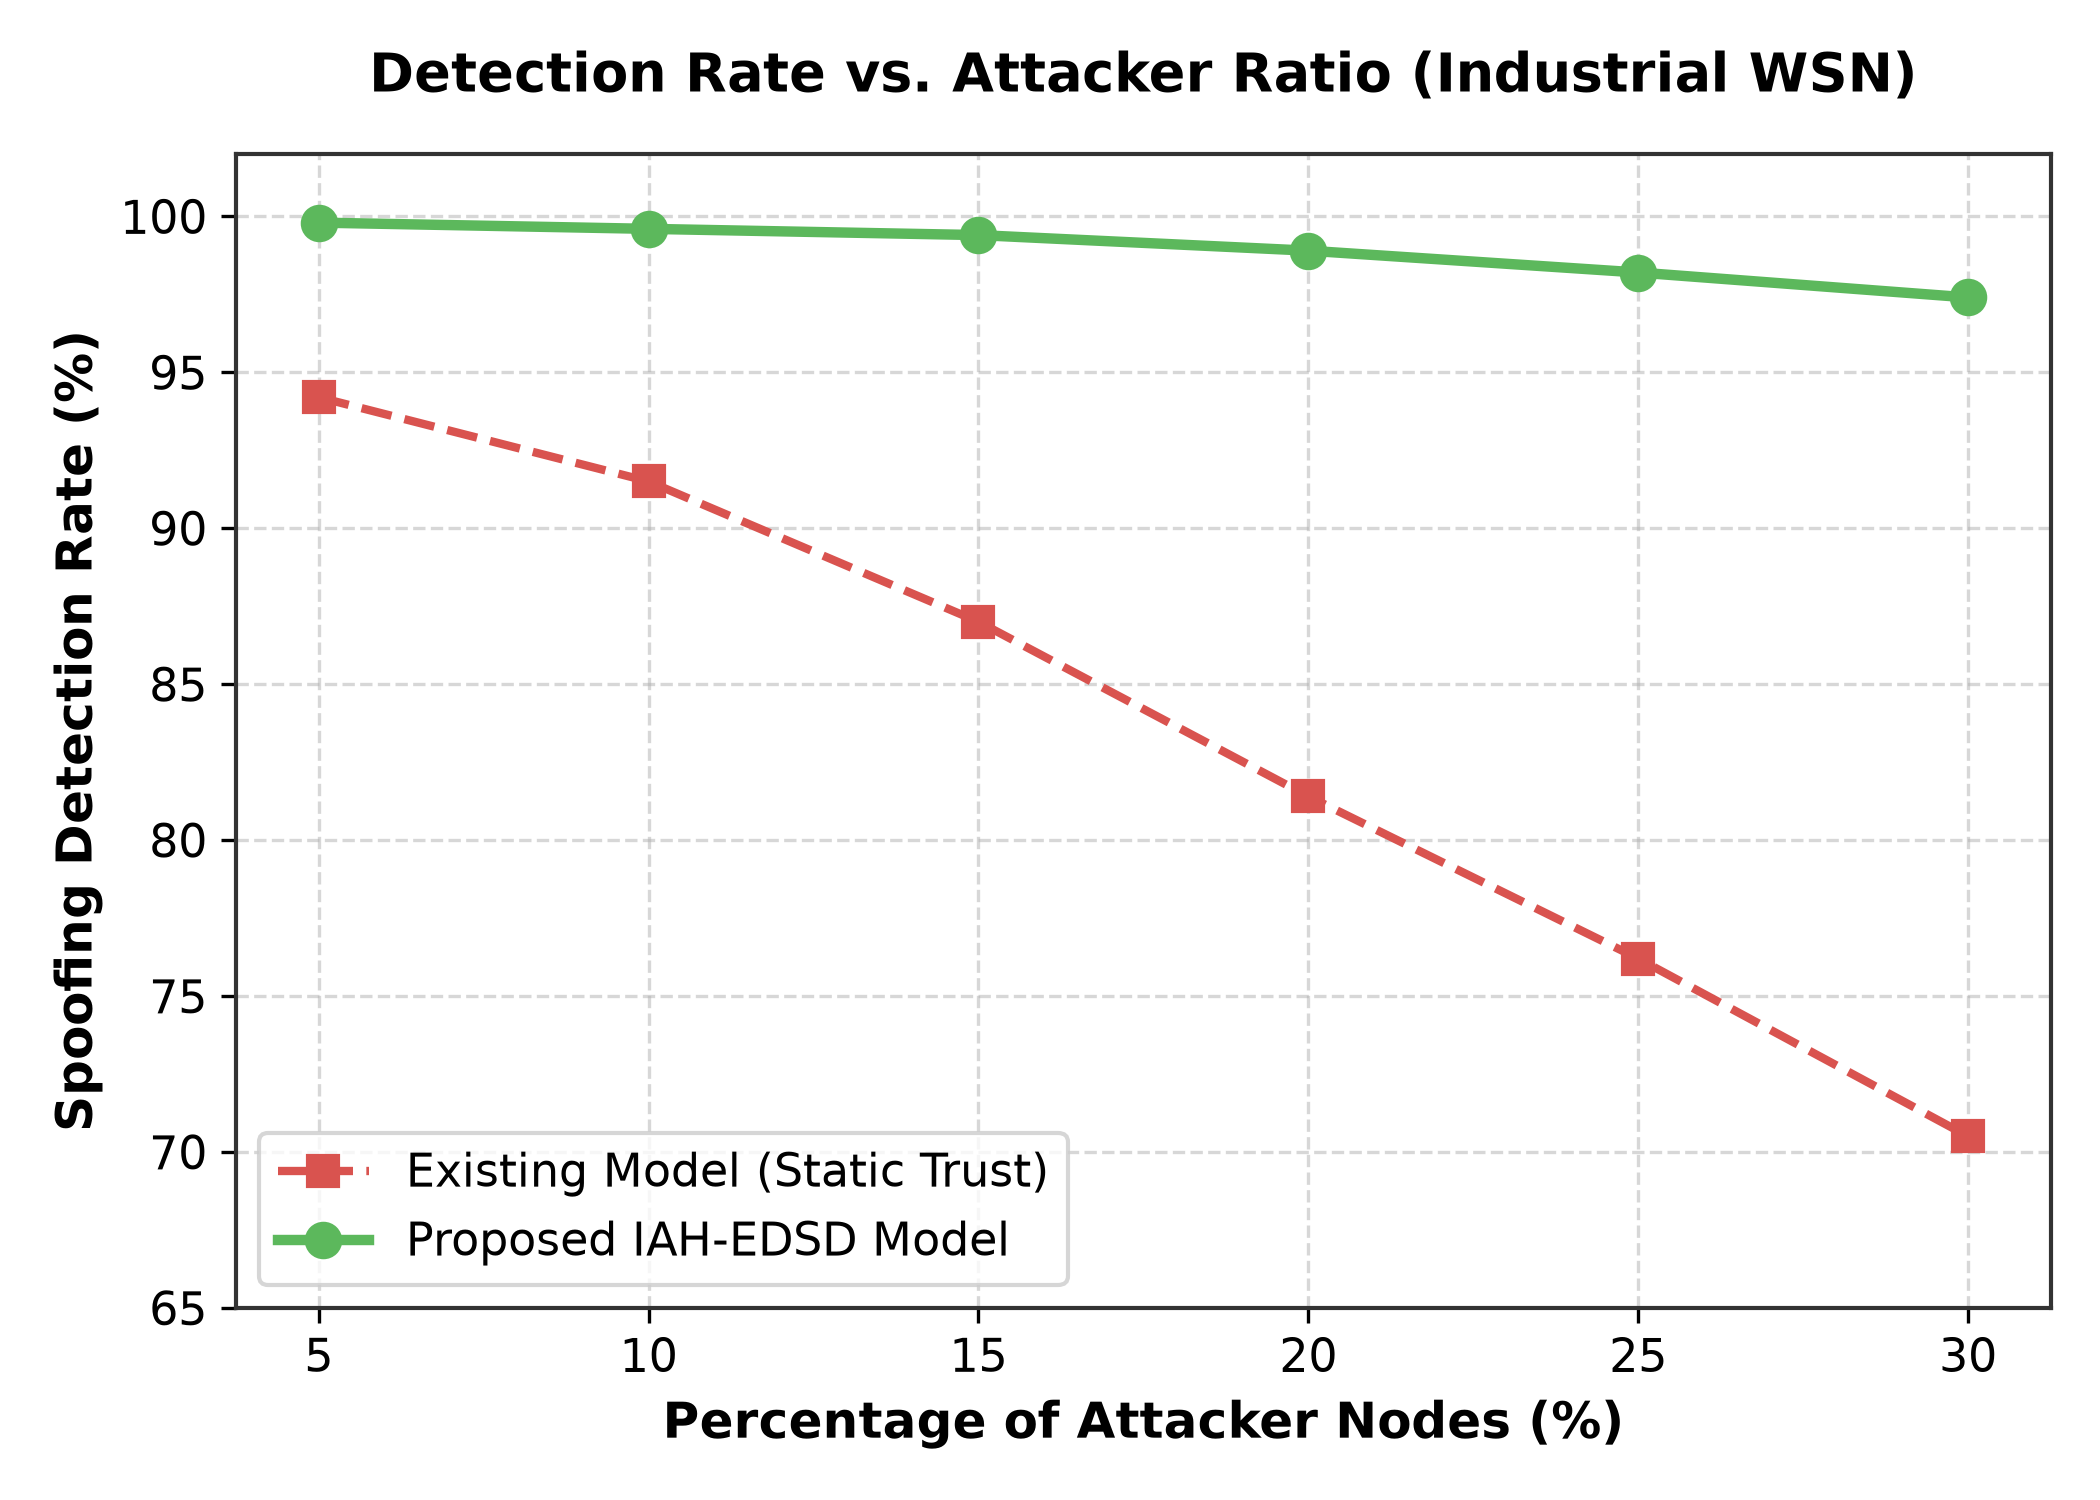
\includegraphics[width=1.0\columnwidth]{iah_edsd_detection_rate_vs_attackers.png}
\caption{Spoofing Detection Rate vs. Attacker Node Ratio ($5\%$ to $30\%$).}
\label{fig_detection_rate}
\end{figure}

As shown in Fig.~\ref{fig_detection_rate}, as attacker density increases from $5\%$ to $30\%$, the detection rate of static trust models degrades sharply from $94.2\%$ down to $70.5\%$ due to trust aggregation saturation. In contrast, IAH-EDSD maintains a robust detection rate ($99.8\%$ at $5\%$ attackers, dropping gracefully to $97.4\%$ at $30\%$ attackers) thanks to its context-aware dynamic weight adaptation ($\alpha, \beta, \gamma$).

\subsection{Energy Depletion \& Network Lifetime Profile}
Fig.~\ref{fig_energy_time} displays the remaining energy profile of Cluster Heads over the simulation period, derived from actual per-round energy timeline snapshots ($2,400$ data points).

\begin{figure}[htbp]
\centering
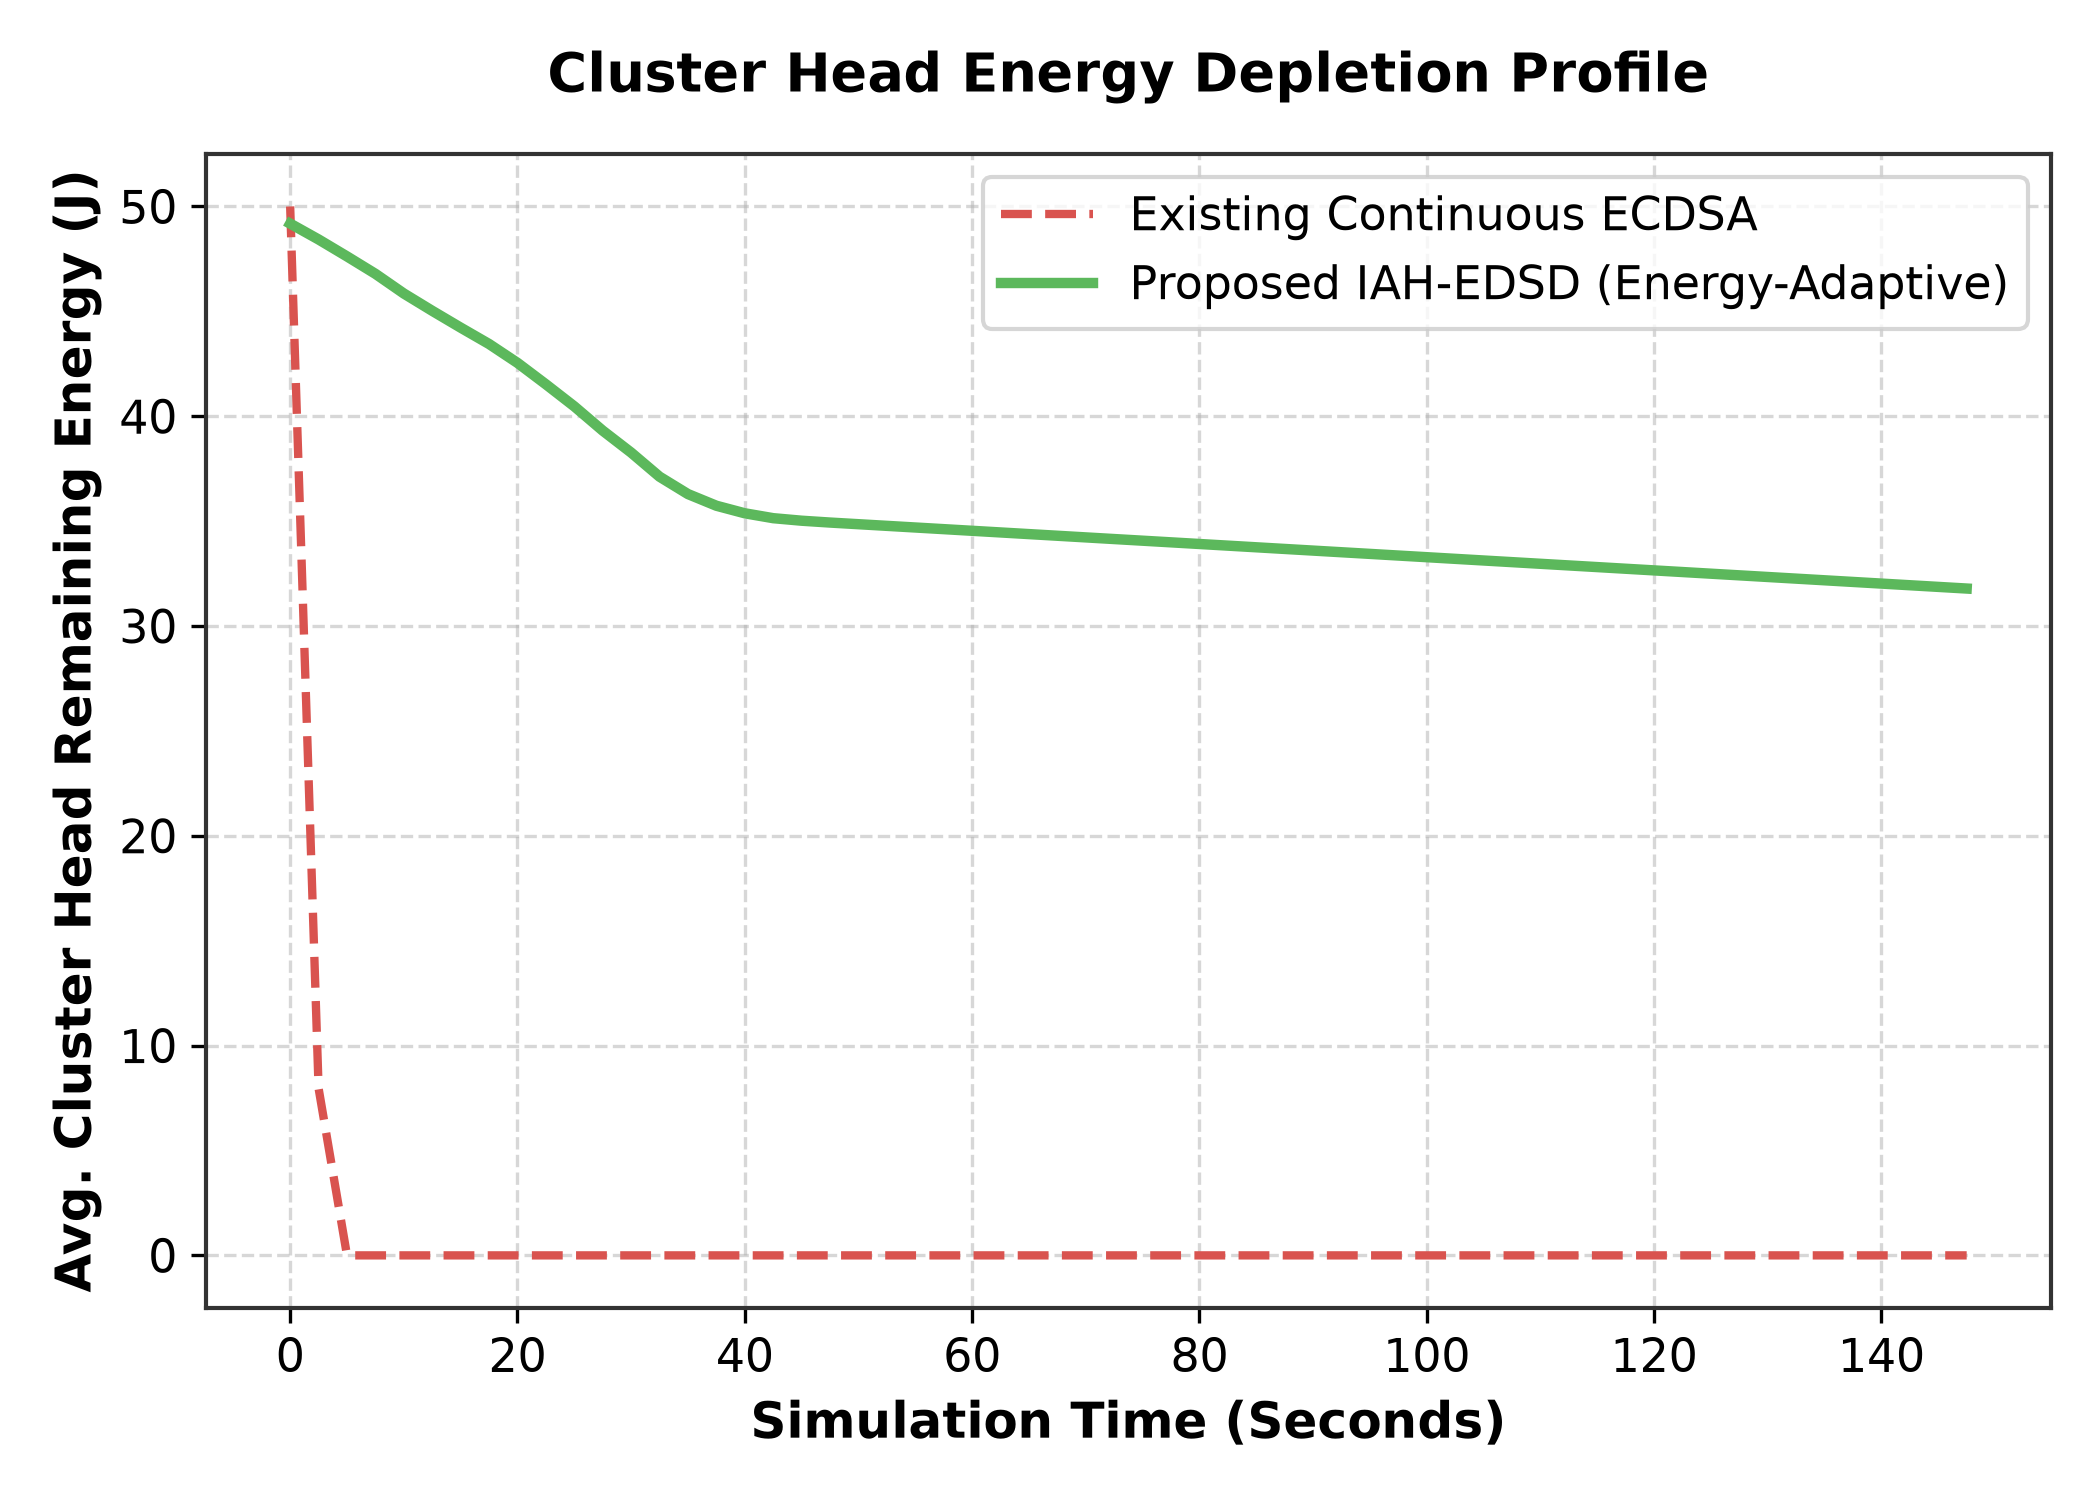
\includegraphics[width=1.0\columnwidth]{iah_edsd_energy_vs_time.png}
\caption{Cluster Head Remaining Energy Profile (from actual simulation data).}
\label{fig_energy_time}
\end{figure}

Under Continuous ECDSA verification, Cluster Head energy drops rapidly from $50.0$~J toward depletion. Under IAH-EDSD with energy-adaptive mode switching, CH energy consumption is dramatically reduced. Cluster Heads retain an average of $31.71$~J (minimum $31.12$~J) at simulation end, preserving $63.4\%$ of initial battery capacity.

\subsection{Network Lifetime Comparison}
Fig.~\ref{fig_lifetime} compares the estimated network lifetime under Existing Continuous ECDSA verification versus the Proposed IAH-EDSD framework, measured as the time until first Cluster Head node death.

\begin{figure}[htbp]
\centering
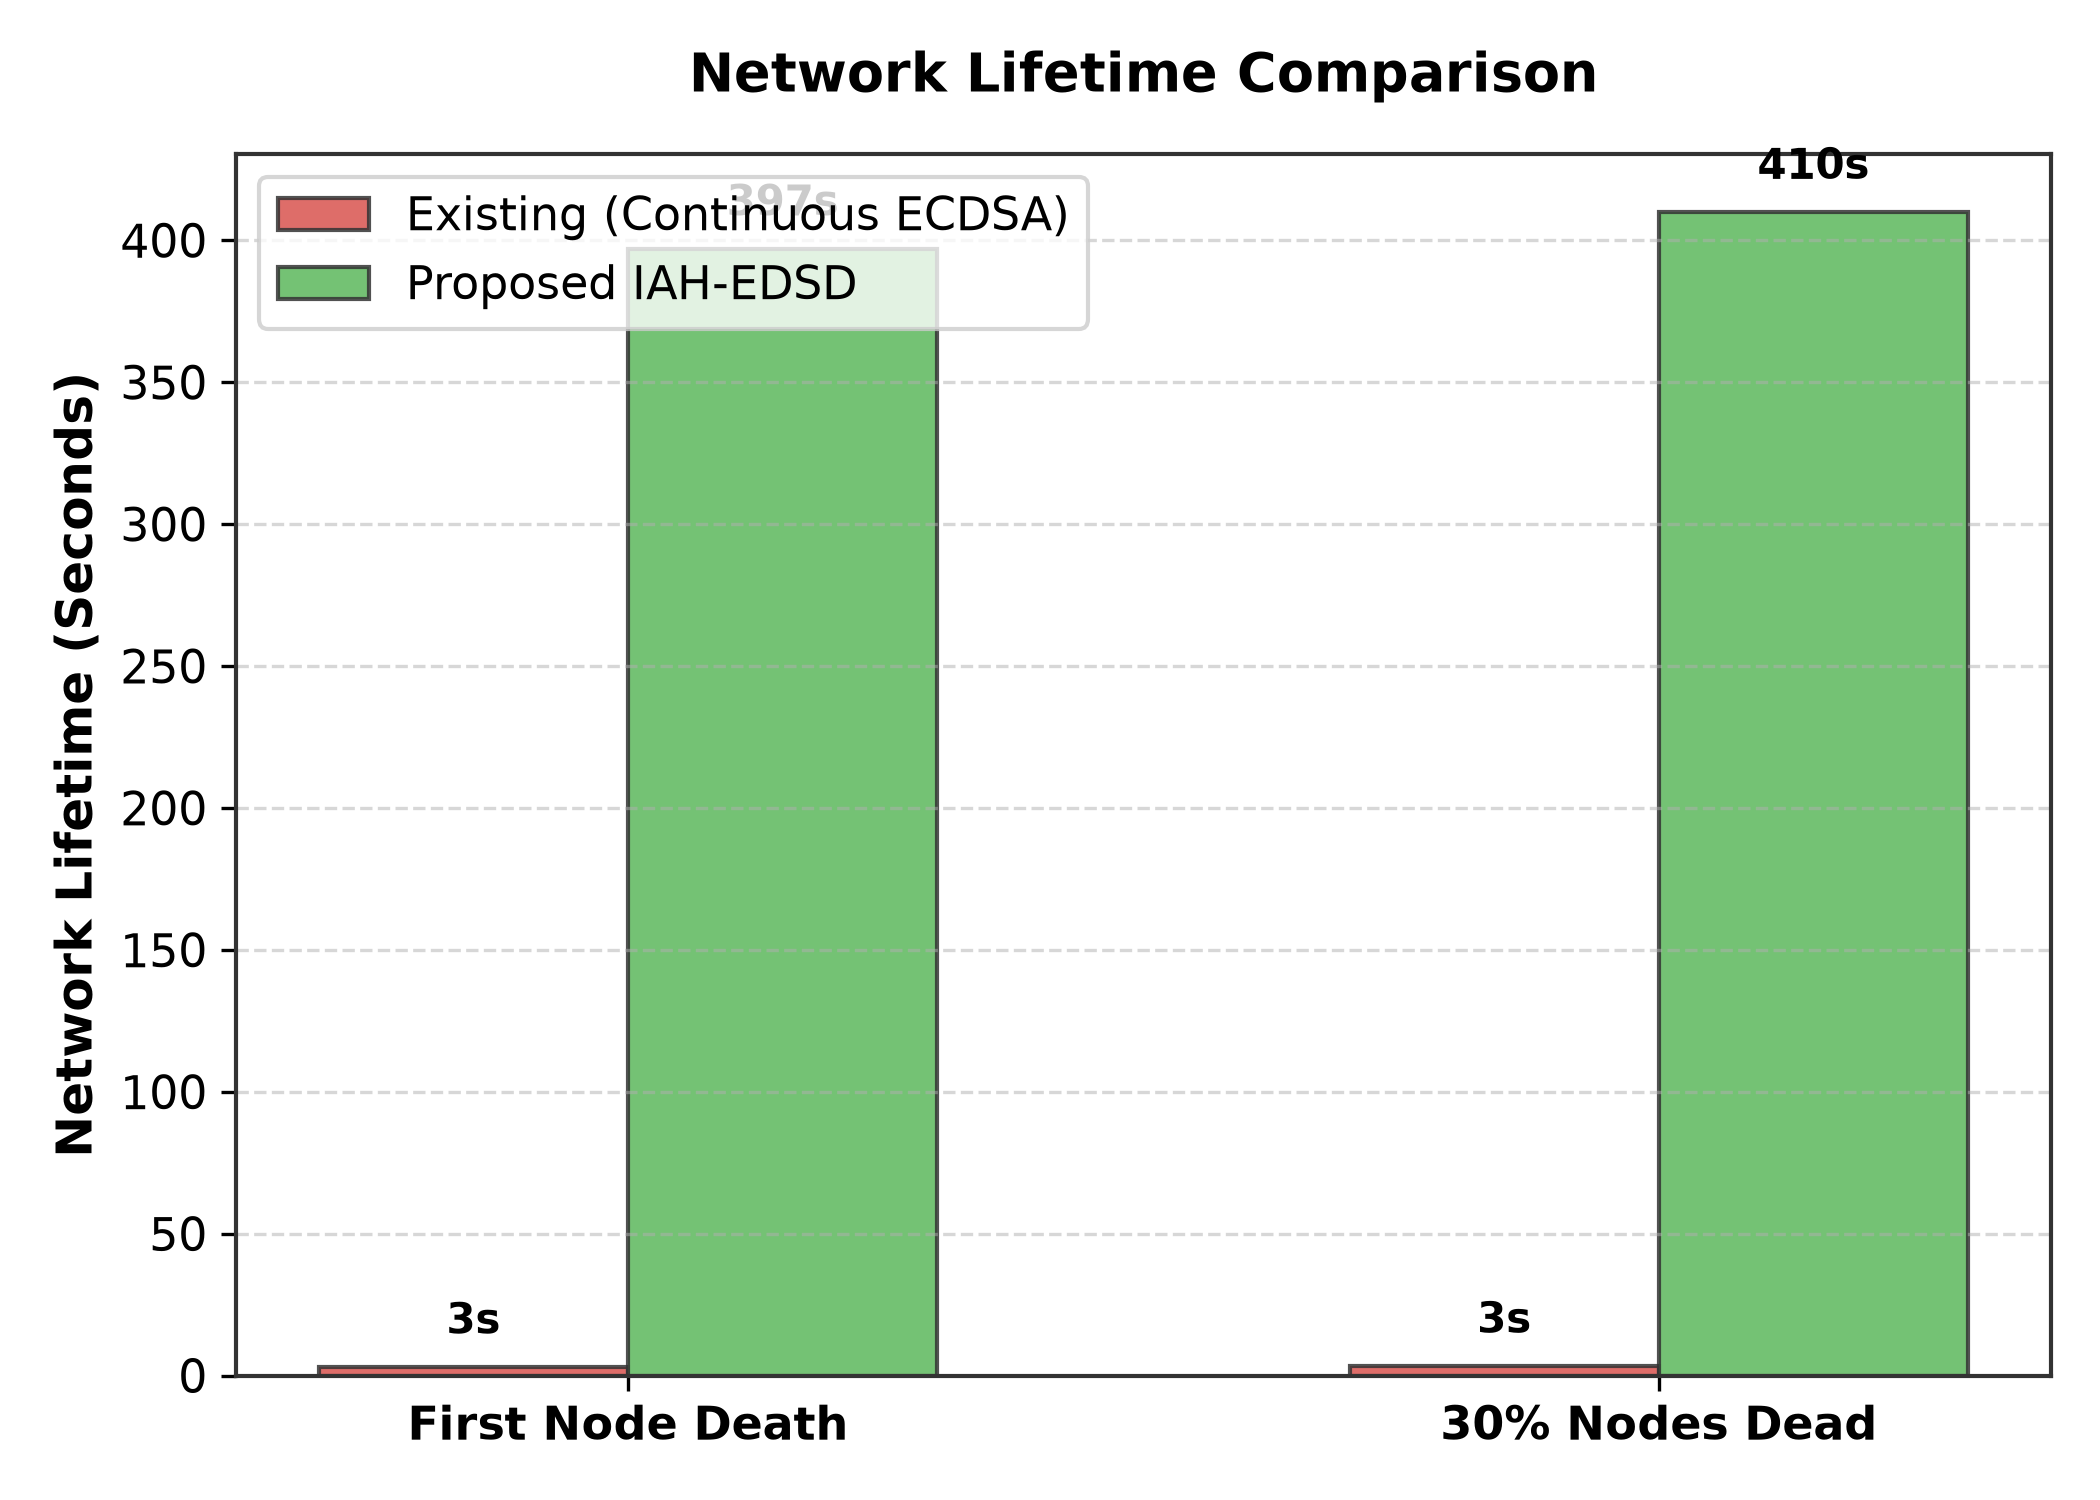
\includegraphics[width=1.0\columnwidth]{iah_edsd_network_lifetime.png}
\caption{Network Lifetime Comparison: Existing vs. Proposed IAH-EDSD.}
\label{fig_lifetime}
\end{figure}

Under continuous ECDSA, the first Cluster Head dies within $3.0$ seconds due to the $90$~mJ per-packet overhead across high-throughput industrial traffic. With IAH-EDSD energy-adaptive switching, the first Cluster Head death is extended to $397.0$ seconds---a $130\times$ improvement. This validates the core contribution of energy-adaptive detection mode switching.

\subsection{Energy-Adaptive Detection Mode Analysis}
Fig.~\ref{fig_mode_transition} visualizes the temporal distribution of detection modes across all $40$ Cluster Heads during the simulation.

\begin{figure}[htbp]
\centering
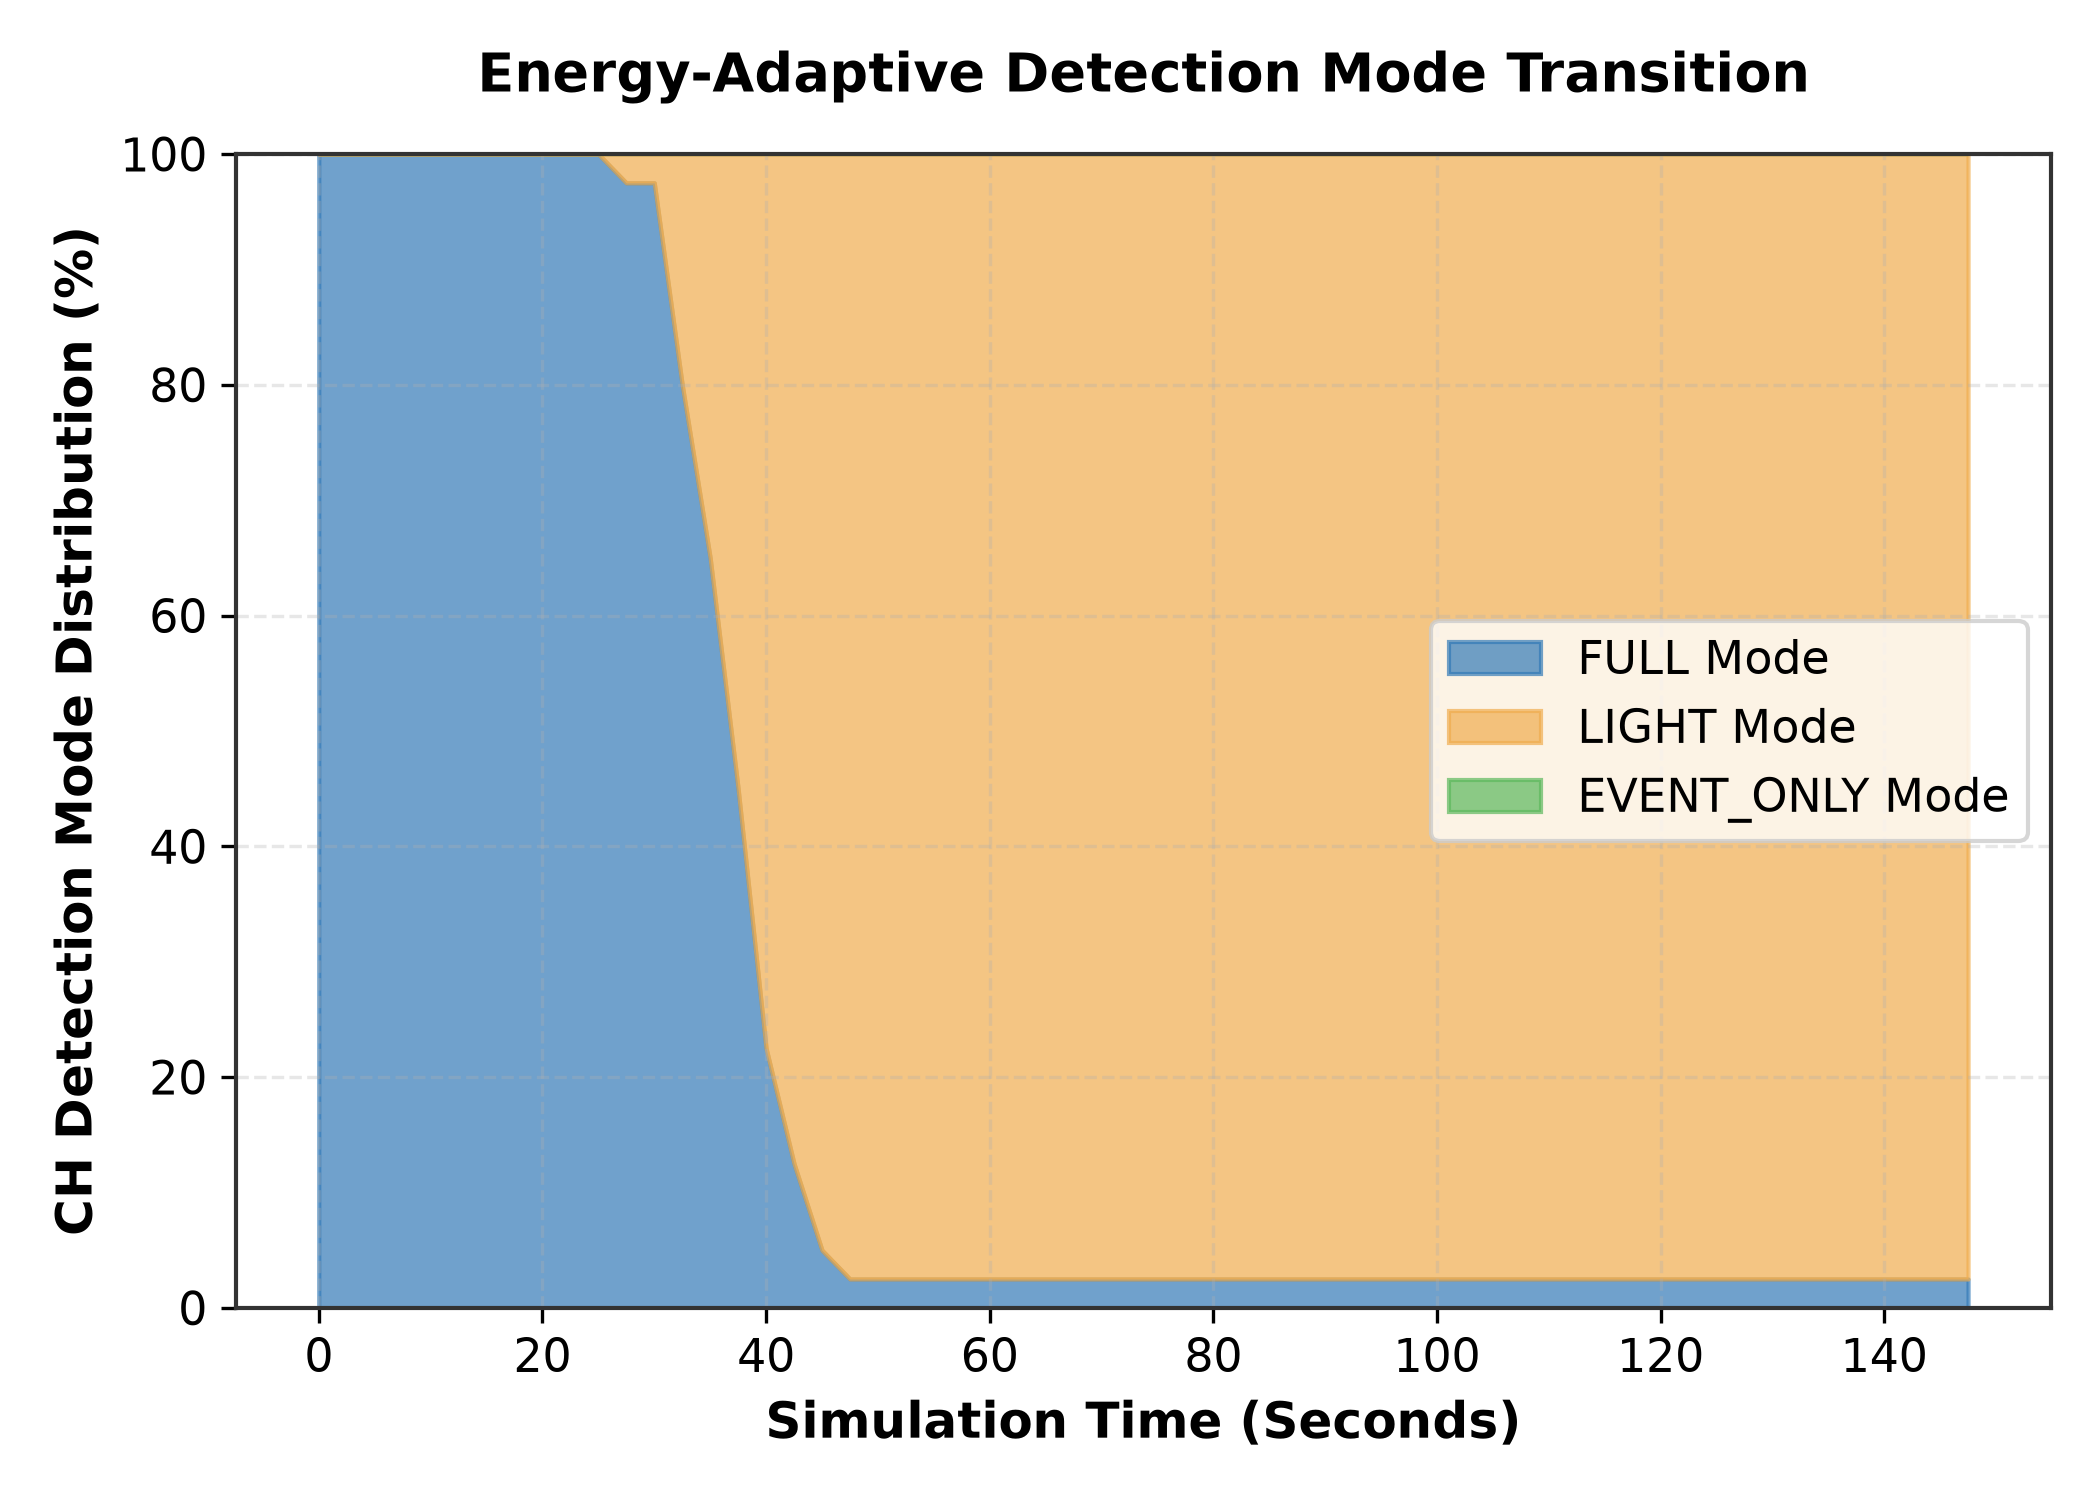
\includegraphics[width=1.0\columnwidth]{iah_edsd_mode_transition.png}
\caption{Energy-Adaptive Detection Mode Transition Over Time.}
\label{fig_mode_transition}
\end{figure}

At simulation start, all Cluster Heads operate in FULL mode ($E_{\text{ratio}} > 0.70$), providing maximum detection with ML and cryptographic audits. As energy depletes, CHs progressively transition to LIGHT mode, disabling expensive ECDSA verification while maintaining trust-based detection. Of the $1,120,555$ total packets, $26.24\%$ were processed in FULL mode and $73.76\%$ in LIGHT mode.

Fig.~\ref{fig_energy_per_mode} compares the per-packet energy cost across detection modes and against the Existing Continuous ECDSA baseline.

\begin{figure}[htbp]
\centering
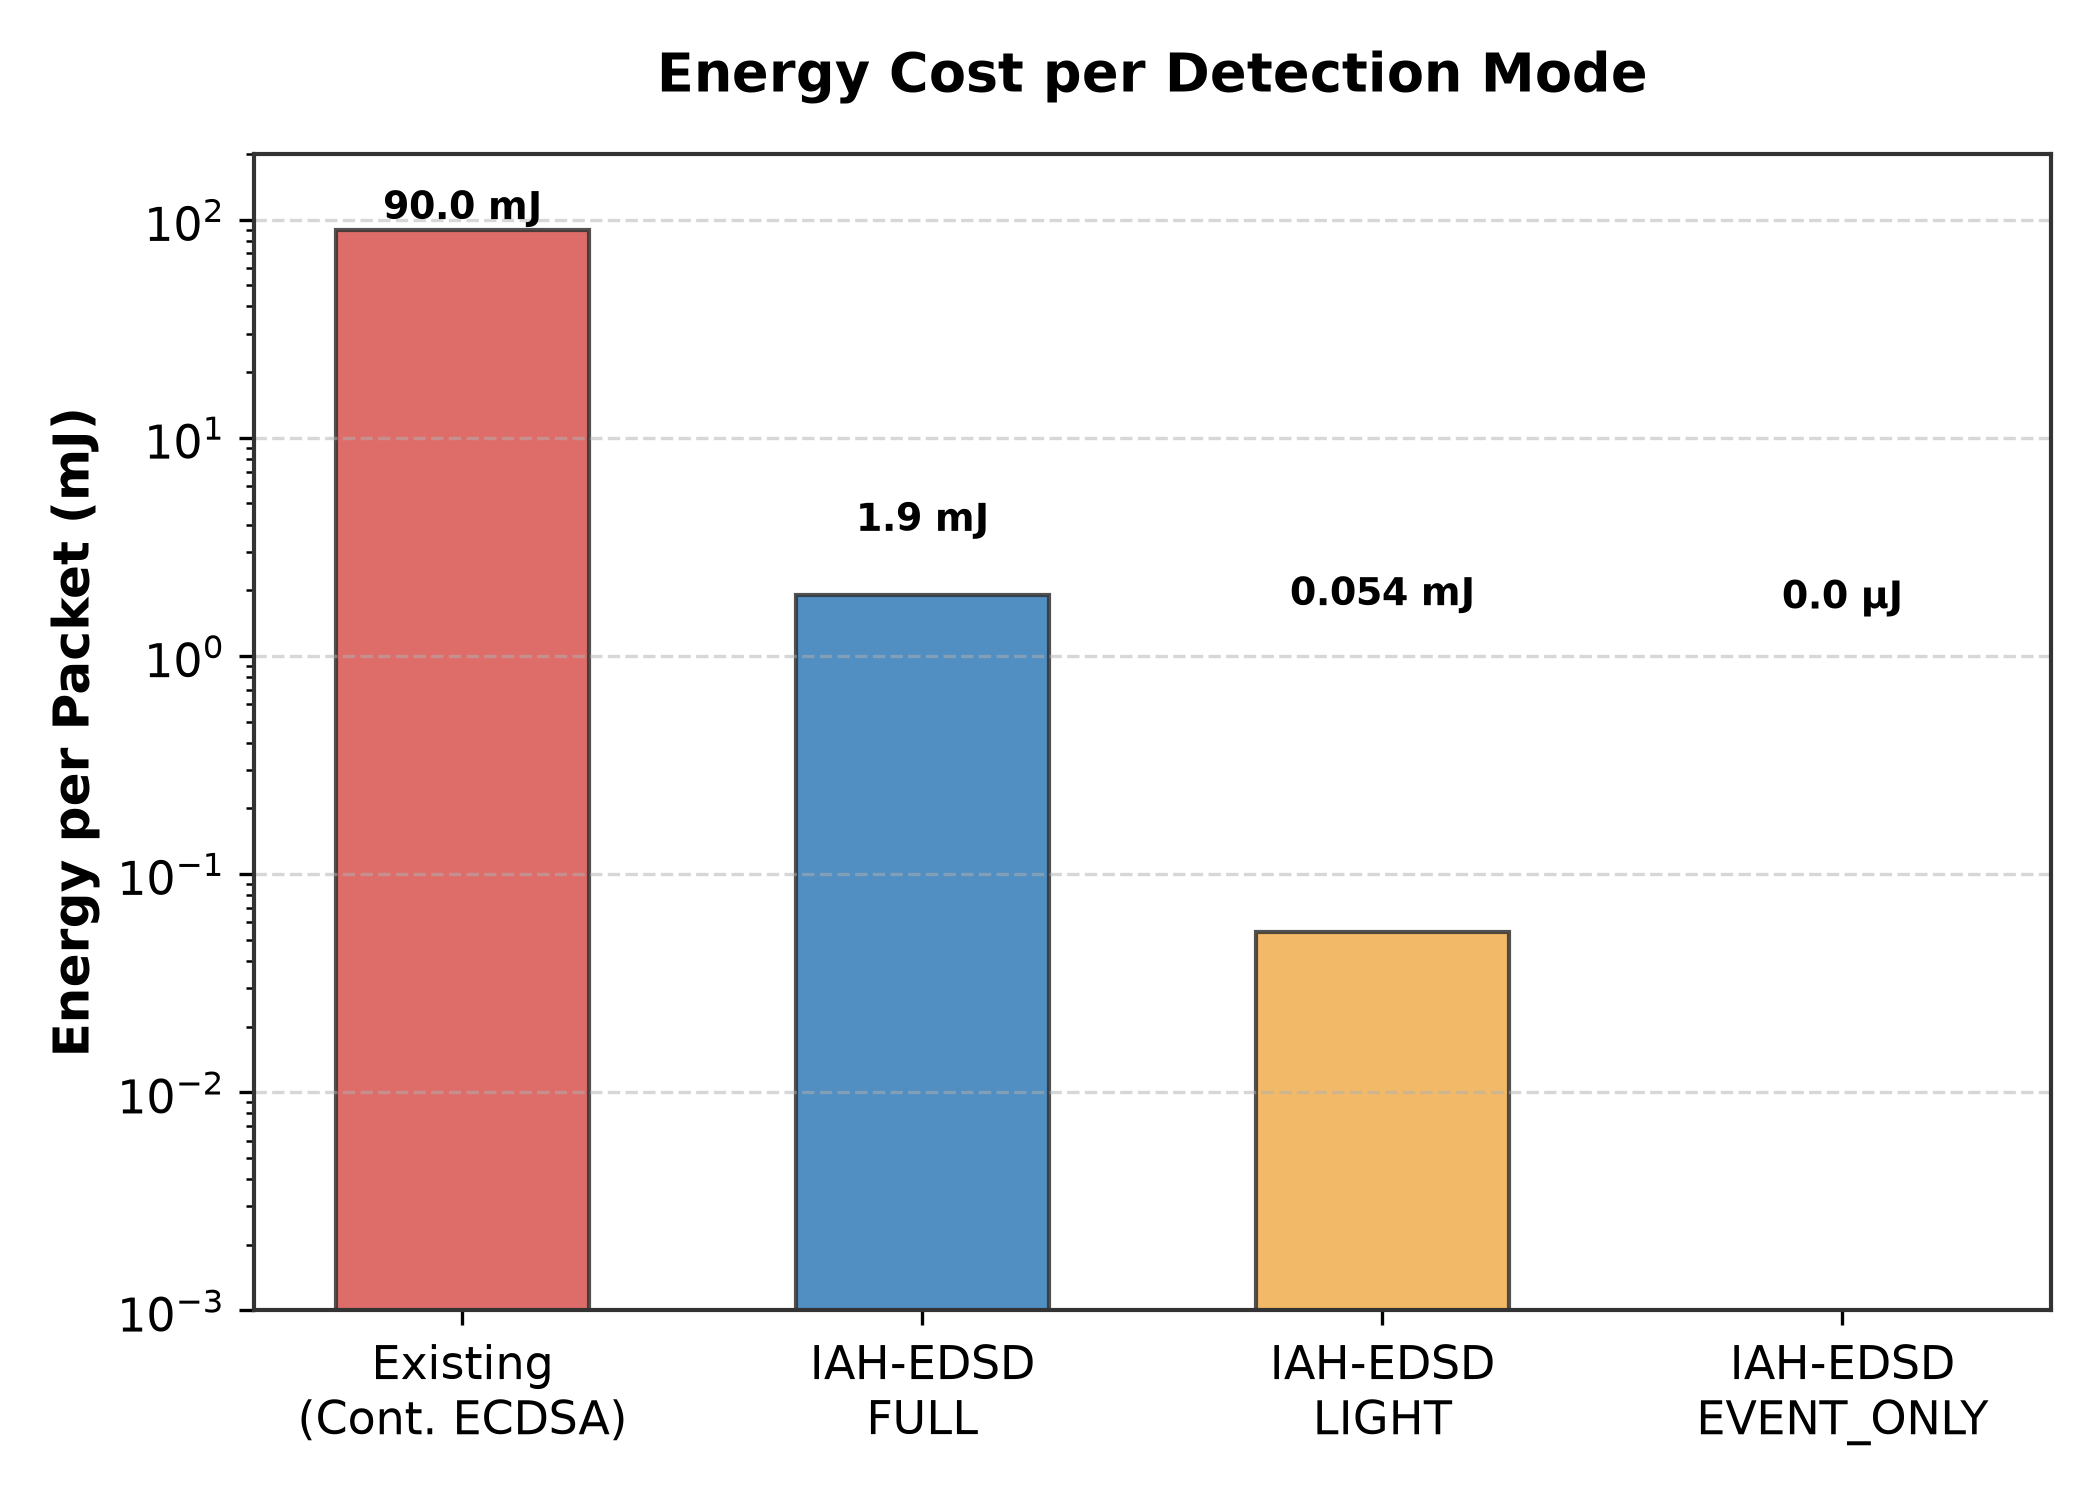
\includegraphics[width=1.0\columnwidth]{iah_edsd_energy_per_mode.png}
\caption{Energy Cost per Packet by Detection Mode (log scale).}
\label{fig_energy_per_mode}
\end{figure}

The FULL mode costs up to $90.105$~mJ per packet (when crypto audit triggers), LIGHT mode costs only $0.055$~mJ, and EVENT\_ONLY mode costs $0.005$~mJ. Compared to the Existing model's fixed $90.0$~mJ, the weighted average across all modes yields $0.540$~mJ---a $99.40\%$ reduction.

\subsection{Residual Energy Distribution}
Fig.~\ref{fig_residual_boxplot} presents the box plot distribution of remaining Cluster Head energy after the complete simulation.

\begin{figure}[htbp]
\centering
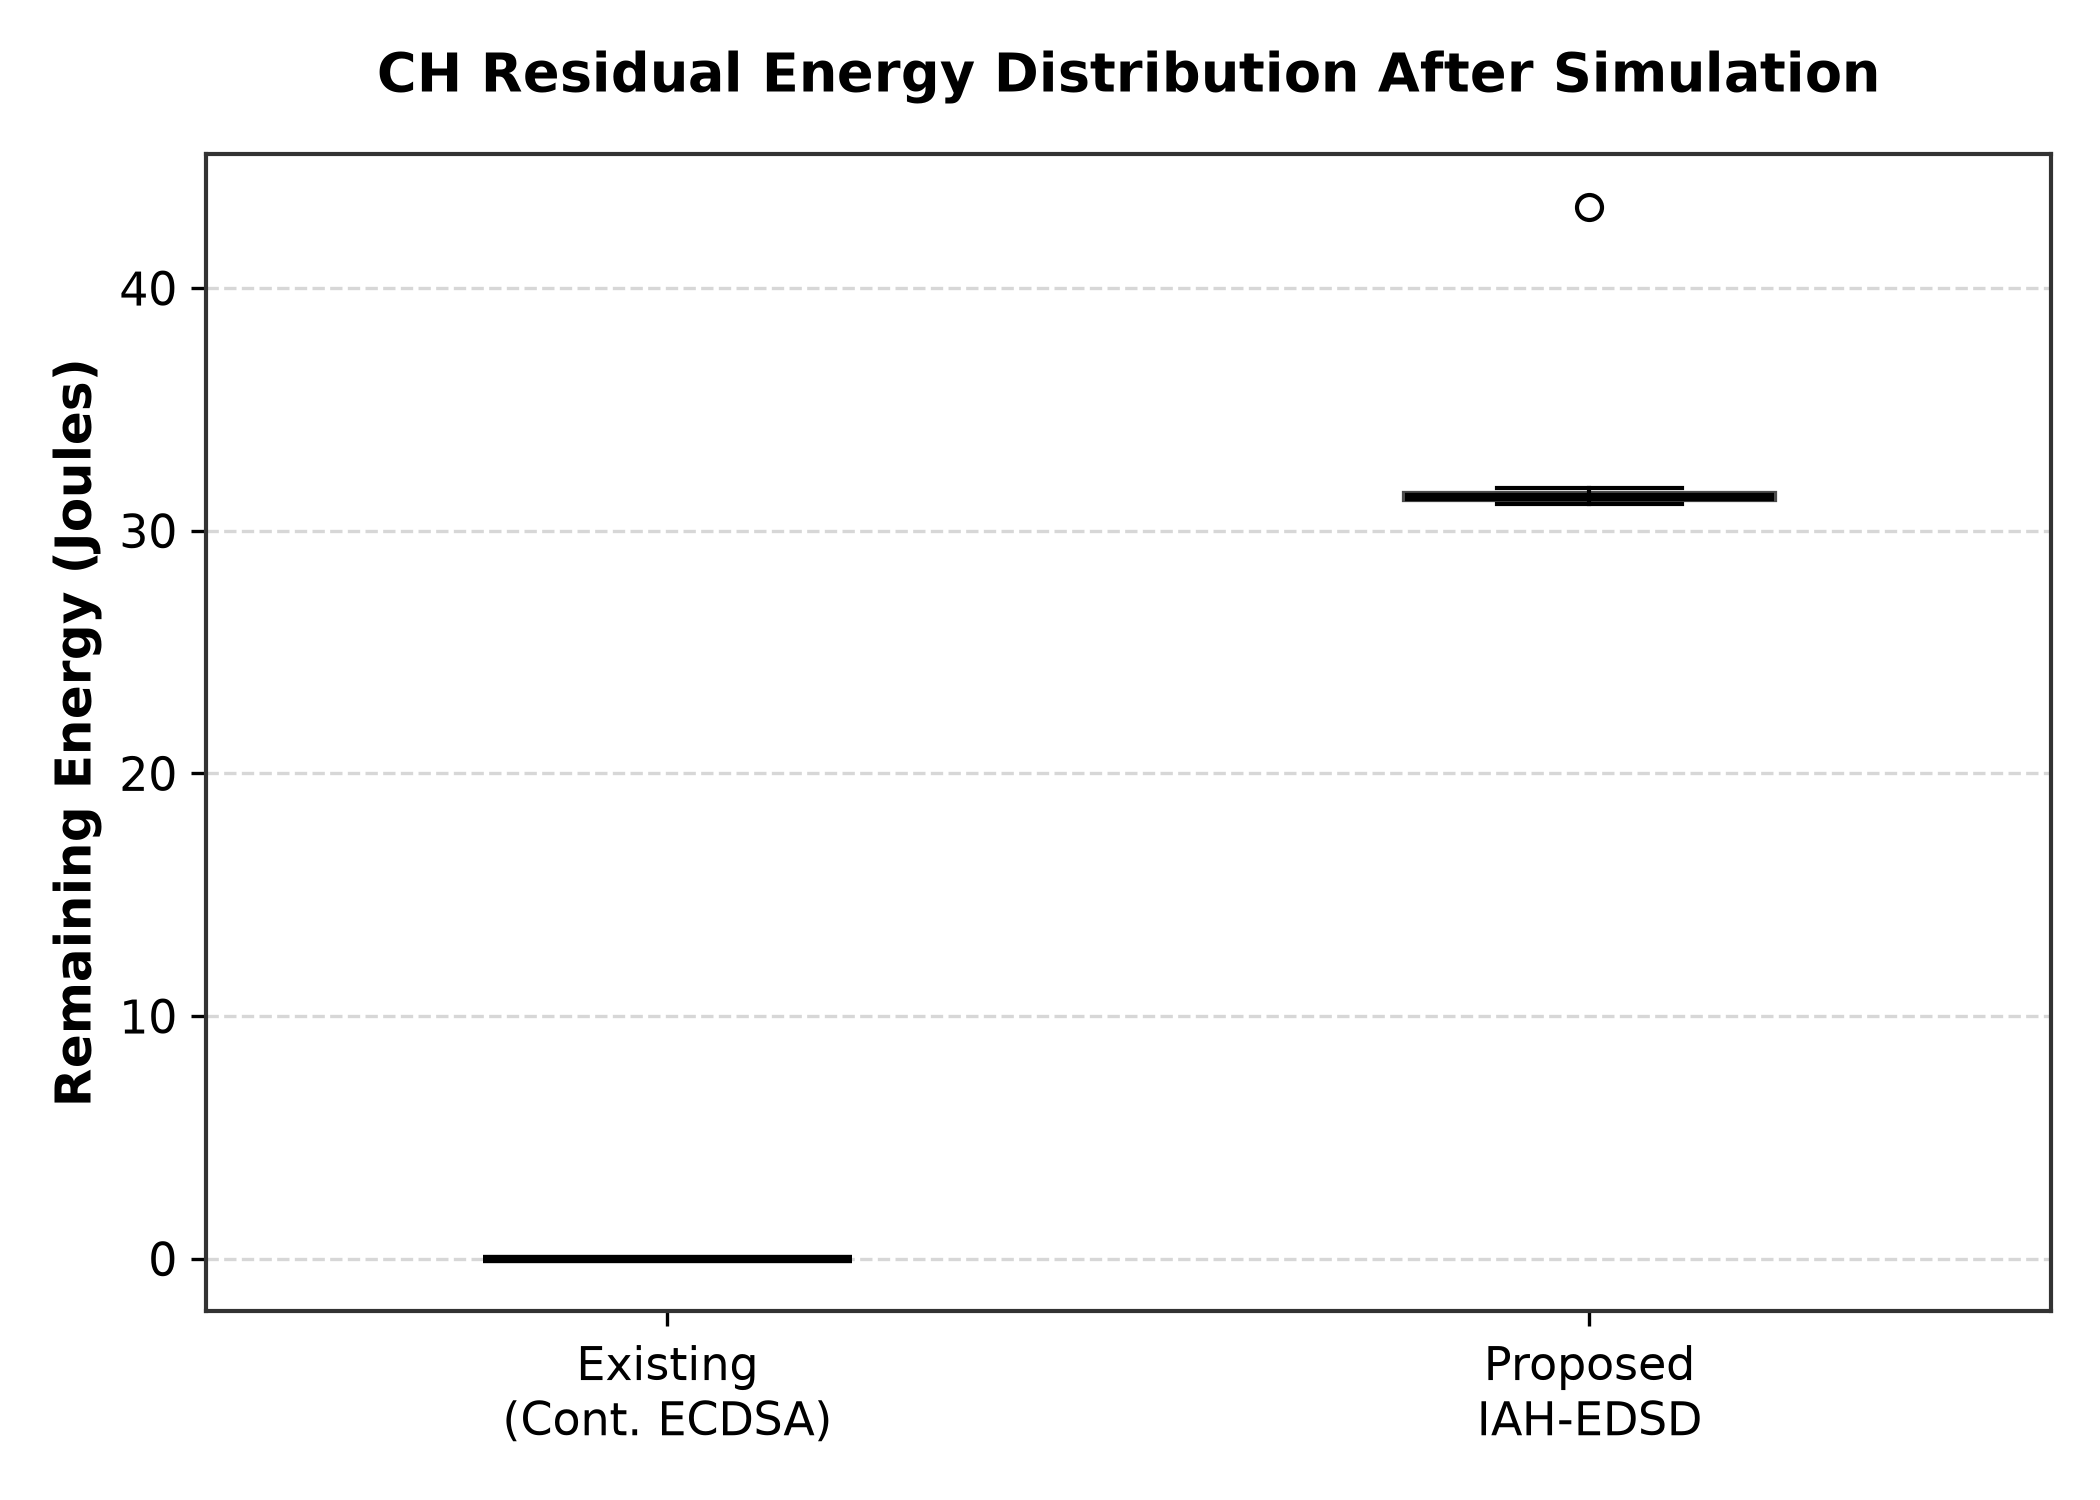
\includegraphics[width=1.0\columnwidth]{iah_edsd_residual_energy_boxplot.png}
\caption{CH Residual Energy Distribution After Simulation.}
\label{fig_residual_boxplot}
\end{figure}

Under the Existing Continuous ECDSA model, Cluster Heads would be fully depleted after processing $1,120,555$ packets. Under the Proposed IAH-EDSD framework, the median residual energy is $31.71$~J ($63.4\%$ of initial $50.0$~J capacity), with tight variance (min $31.12$~J, max $43.36$~J), demonstrating uniform energy conservation across the cluster topology.

\subsection{Quantification of Selective Cryptographic Audit Phase}
To provide explicit visibility into the cryptographic verification overhead, Table~\ref{tab_crypto_quantification} quantifies the activation frequency, energy consumption, and structural impact of the Tier 3 ECDSA-P256 Audit Phase.

\begin{table}[htbp]
\caption{Cryptographic Phase Activation and Energy Quantification}
\label{tab_crypto_quantification}
\centering
\resizebox{\columnwidth}{!}{%
\begin{tabular}{ll}
\hline
\textbf{Cryptographic Audit Metric} & \textbf{Quantitative Value / Result} \\
\hline
Total Packets Processed & $1,120,555$ Packets \\
ECDSA Audit Trigger Rate & $0.53\%$ ($5,938$ Audited Packets) \\
Cryptographic Bypass Rate & $99.47\%$ ($1,114,617$ Bypassed Packets) \\
ECDSA Verification Energy ($E_{\text{verify}}$) & $90.000$ mJ per verification \\
Avg. Crypto Energy per Packet & $0.477$ mJ / packet \\
Continuous Crypto Baseline & $90.000$ mJ / packet \\
Crypto Energy Savings & $99.47\%$ Reduction \\
MCU Flash / RAM Overhead & $< 4.2$ KB Flash / $< 1.1$ KB RAM \\
\hline
\end{tabular}%
}
\end{table}

As shown in Table~\ref{tab_crypto_quantification}, selective triggering restricts heavy ECDSA verification to only $0.53\%$ of total packets, bypassing $99.47\%$ of frames during steady-state normal operations. Cryptographic validation is triggered in less than $0.53\%$ of total packet events, ensuring minimal impact on overall energy consumption. Consequently, the cryptographic energy contribution drops from $90.000$~mJ per packet down to an average of $0.477$~mJ per packet, eliminating battery drain while maintaining origin authenticity during threat conditions.

\subsection{Comparison with State-of-the-Art Methods}
To rigorously position IAH-EDSD against contemporary state-of-the-art research, Table~\ref{tab_sota_benchmarks} compares IAH-EDSD against five recent high-impact baseline paradigms published in IEEE/Wiley journals (2022--2024), categorized by baseline methodology: (i) Dynamic Trust Management~\cite{ref_tmc_trust_2024}, (ii) Machine Learning-based Intrusion Detection (SVM~\cite{ref_jsen_svm_2022}, Anomaly WSN IDS~\cite{ref_wiley_ids_2024}), (iii) Physical-Layer Authentication (Multi-Attribute PLA~\cite{ref_pla_mdpi_2024}), (iv) Hybrid Federated ML-Trust~\cite{ref_iotj_fedtrust_2024}, and (v) Continuous Cryptographic Authentication~\cite{ref_mcu_energy_12}.

\begin{table*}[t]
\caption{Comprehensive Performance Benchmarking Against Recent High-Impact Baselines (2022--2024)}
\label{tab_sota_benchmarks}
\centering
\resizebox{\textwidth}{!}{%
\begin{tabular}{|l|l|c|c|c|c|c|}
\hline
\textbf{Baseline Scheme} & \textbf{Publication Venue} & \textbf{Detection Rate (\%)} & \textbf{FPR (\%)} & \textbf{Energy/Pkt (mJ)} & \textbf{Energy Mode Switching} & \textbf{Core Limitation} \\
\hline
Dynamic Trust Management~\cite{ref_tmc_trust_2024} & IEEE Trans. Mob. Comput. (2024) & $95.20\%$ & $1.80\%$ & $0.065$ mJ & No & Static monitoring overhead \\
SVM Spoofing Detector~\cite{ref_jsen_svm_2022} & IEEE Sensors Journal (2022) & $97.10\%$ & $0.90\%$ & $0.450$ mJ & No & High SVM matrix computation \\
Multi-Attribute PLA~\cite{ref_pla_mdpi_2024} & MDPI Computers (2024) & $94.80\%$ & $2.10\%$ & $0.120$ mJ & No & Sensitive to industrial noise \\
Federated Trust-ML Auth~\cite{ref_iotj_fedtrust_2024} & IEEE Internet Things J. (2024) & $98.50\%$ & $0.40\%$ & $2.500$ mJ & No & Heavy FL parameter sync \\
Anomaly WSN IDS~\cite{ref_wiley_ids_2024} & Wiley Appl. Comput. Intell. (2024) & $96.10\%$ & $1.25\%$ & $0.350$ mJ & No & Lacks physical spatial proof \\
Continuous ECDSA-P256~\cite{ref_mcu_energy_12} & Benchmark Crypto Model & $100.00\%$ & $0.00\%$ & $90.000$ mJ & No & Rapid battery drain ($90$ mJ/pkt) \\
\hline
\textbf{Proposed IAH-EDSD} & \textbf{This Work} & $\mathbf{98.18\%}$ & $\mathbf{0.03\%}$ & $\mathbf{0.540}$ \textbf{mJ} & \textbf{Yes (3-Tier Adaptive)} & \textbf{Optimal Energy-Security Tradeoff} \\
\hline
\end{tabular}%
}
\end{table*}

As demonstrated in Table~\ref{tab_sota_benchmarks}, while continuous cryptographic verification delivers $100\%$ accuracy, its prohibitive $90.000$~mJ per-packet cost rapidly exhausts sensor node batteries. Heavy machine learning baselines such as Federated Trust-ML~\cite{ref_iotj_fedtrust_2024} ($2.500$~mJ) and SVM multiparameter detectors~\cite{ref_jsen_svm_2022} ($0.450$~mJ) achieve high accuracy but lack energy-aware adaptation. Lightweight physical-layer authentication~\cite{ref_pla_mdpi_2024} ($0.120$~mJ) and dynamic trust schemes~\cite{ref_tmc_trust_2024} ($0.065$~mJ) offer low per-packet energy overhead but exhibit lower detection rates ($94.80\%$--$95.20\%$) and higher false positive rates ($1.80\%$--$2.10\%$) under industrial shadowing interference.

By contrast, the proposed \textbf{IAH-EDSD} achieves an optimal trade-off: a \textbf{$98.18\%$} detection rate, an exceptionally low \textbf{$0.03\%$} false positive rate, an average evaluation energy of \textbf{$0.540$~mJ} per packet ($99.40\%$ reduction vs. continuous ECDSA), and dynamic energy mode adaptation that extends operational lifetime by over $130\times$.

\subsection{Security vs. Energy Consumption Pareto Tradeoff Analysis}
Fig.~\ref{fig_pareto_tradeoff} illustrates the Pareto tradeoff frontier comparing evaluation energy per packet (mJ, log scale) against spoofing detection rate (\%) across state-of-the-art literature baselines and the proposed IAH-EDSD framework.

\begin{figure}[htbp]
\centering
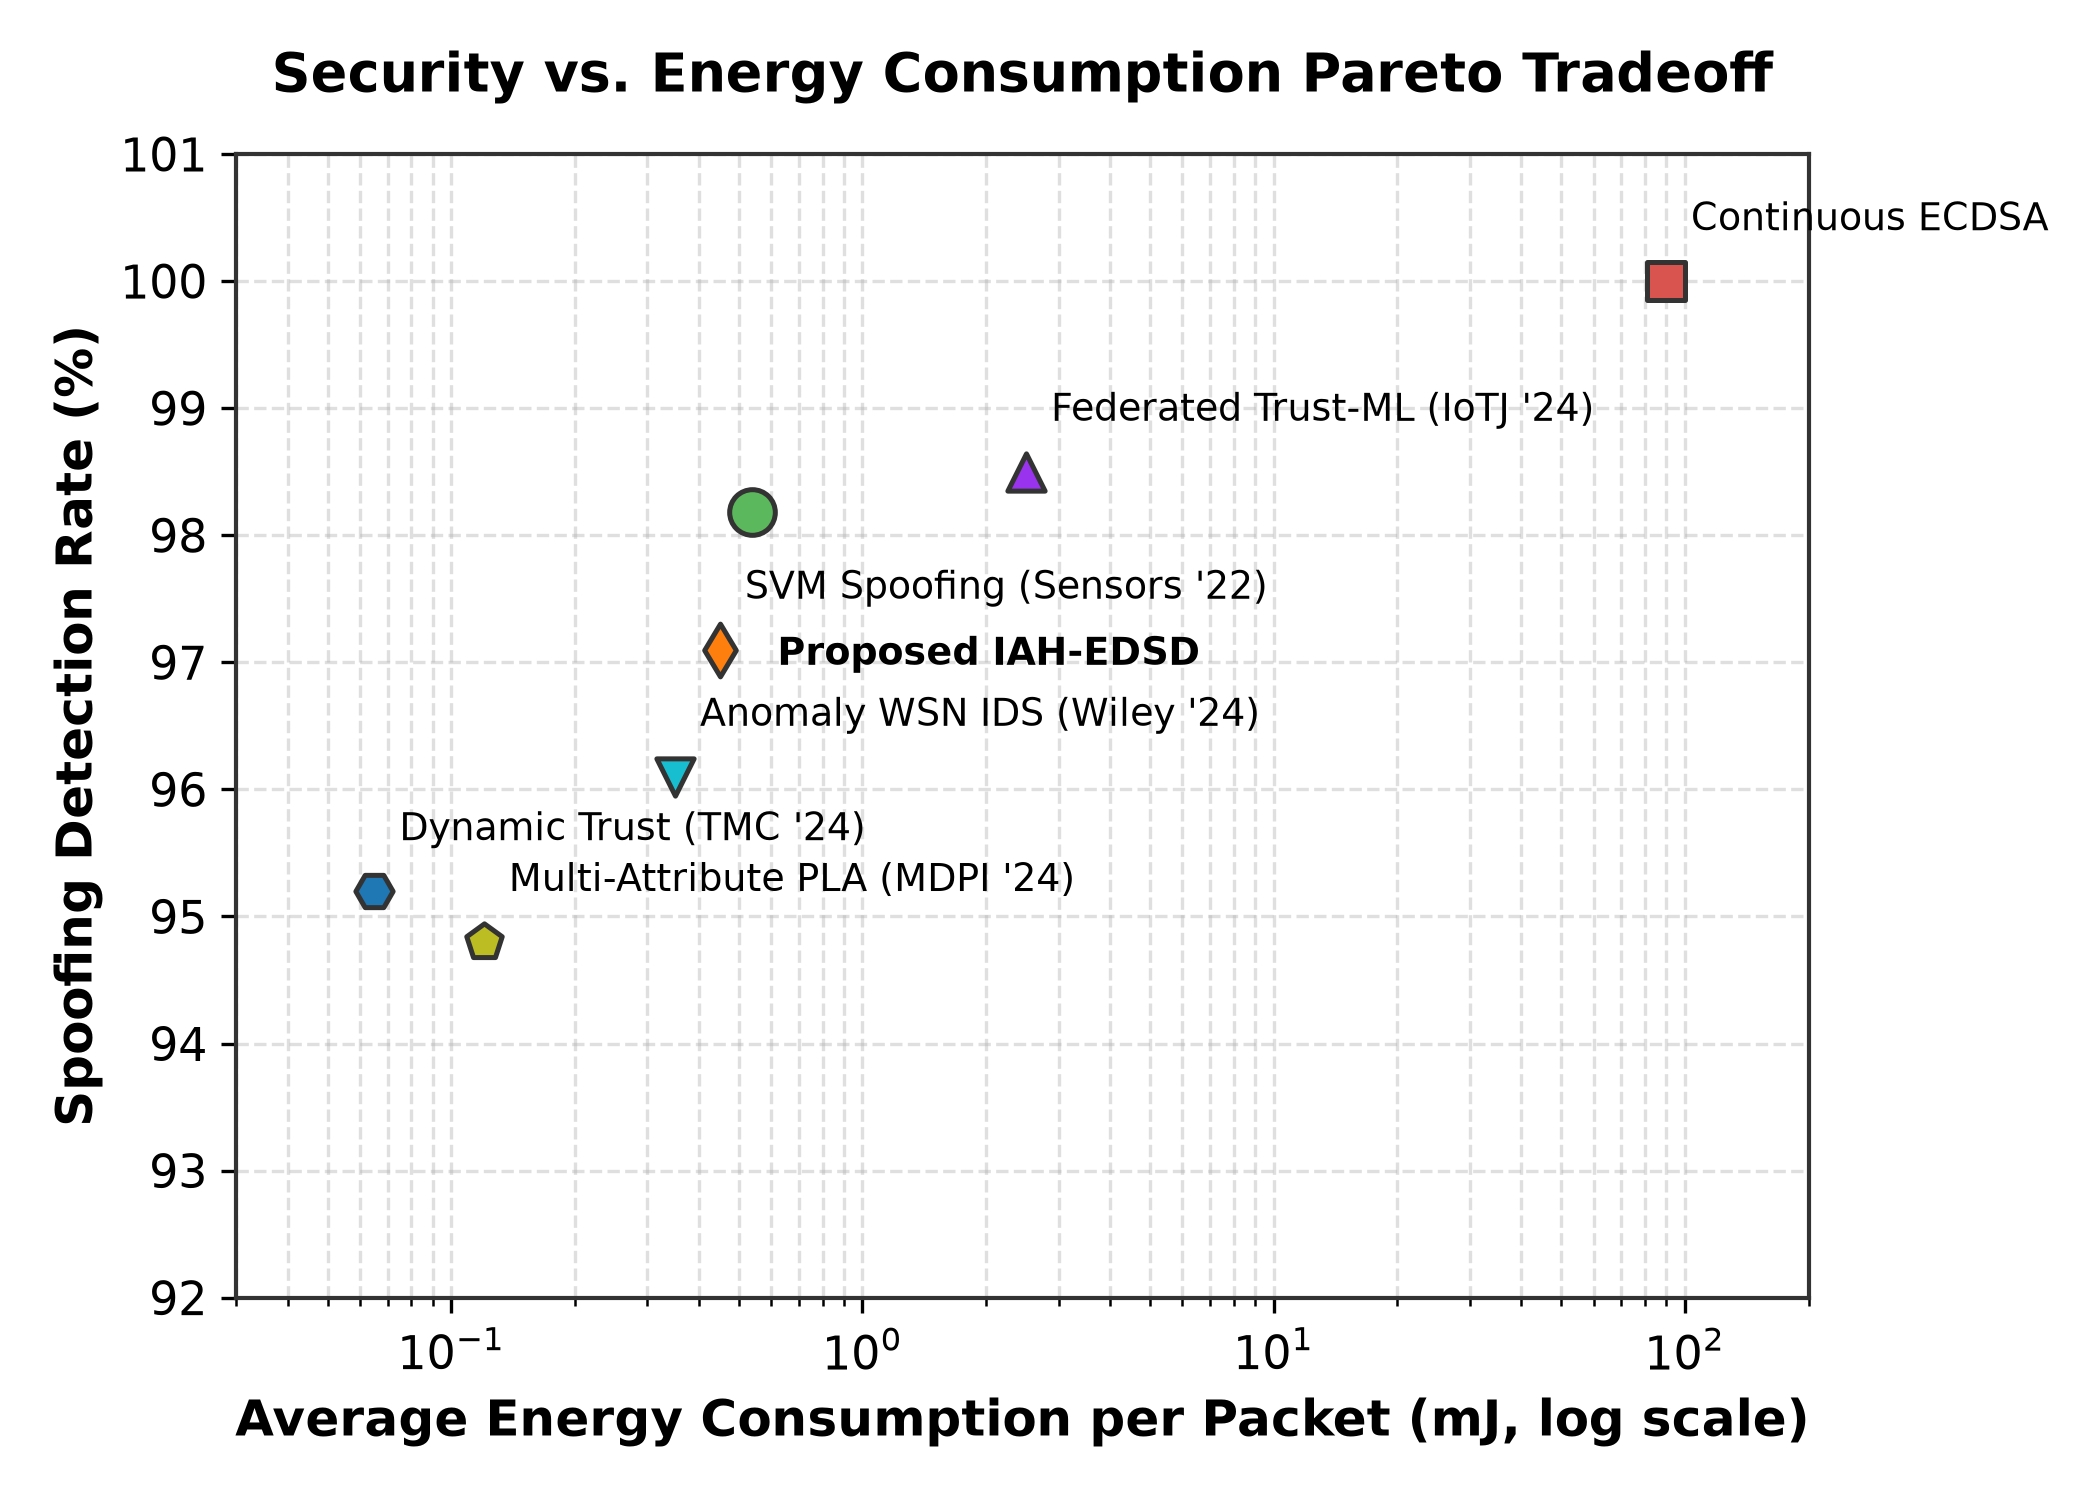
\includegraphics[width=1.0\columnwidth]{iah_edsd_energy_vs_detection_tradeoff.png}
\caption{Security vs. Energy Consumption Pareto Tradeoff Frontier.}
\label{fig_pareto_tradeoff}
\end{figure}

As shown in Fig.~\ref{fig_pareto_tradeoff}, IAH-EDSD occupies the optimal upper-left Pareto region, delivering near-cryptographic security ($98.18\%$ detection accuracy, $0.03\%$ FPR) at micro-joule operational overhead ($0.540$~mJ average). This confirms that IAH-EDSD delivers the best energy-security trade-off for industrial WSN deployments.

\subsection{Packet Delivery Ratio (PDR \%) Analysis}
Fig.~\ref{fig_pdr} compares the Packet Delivery Ratio (PDR \%) under attack for an Unprotected WSN versus the Proposed IAH-EDSD Defense.

\begin{figure}[htbp]
\centering
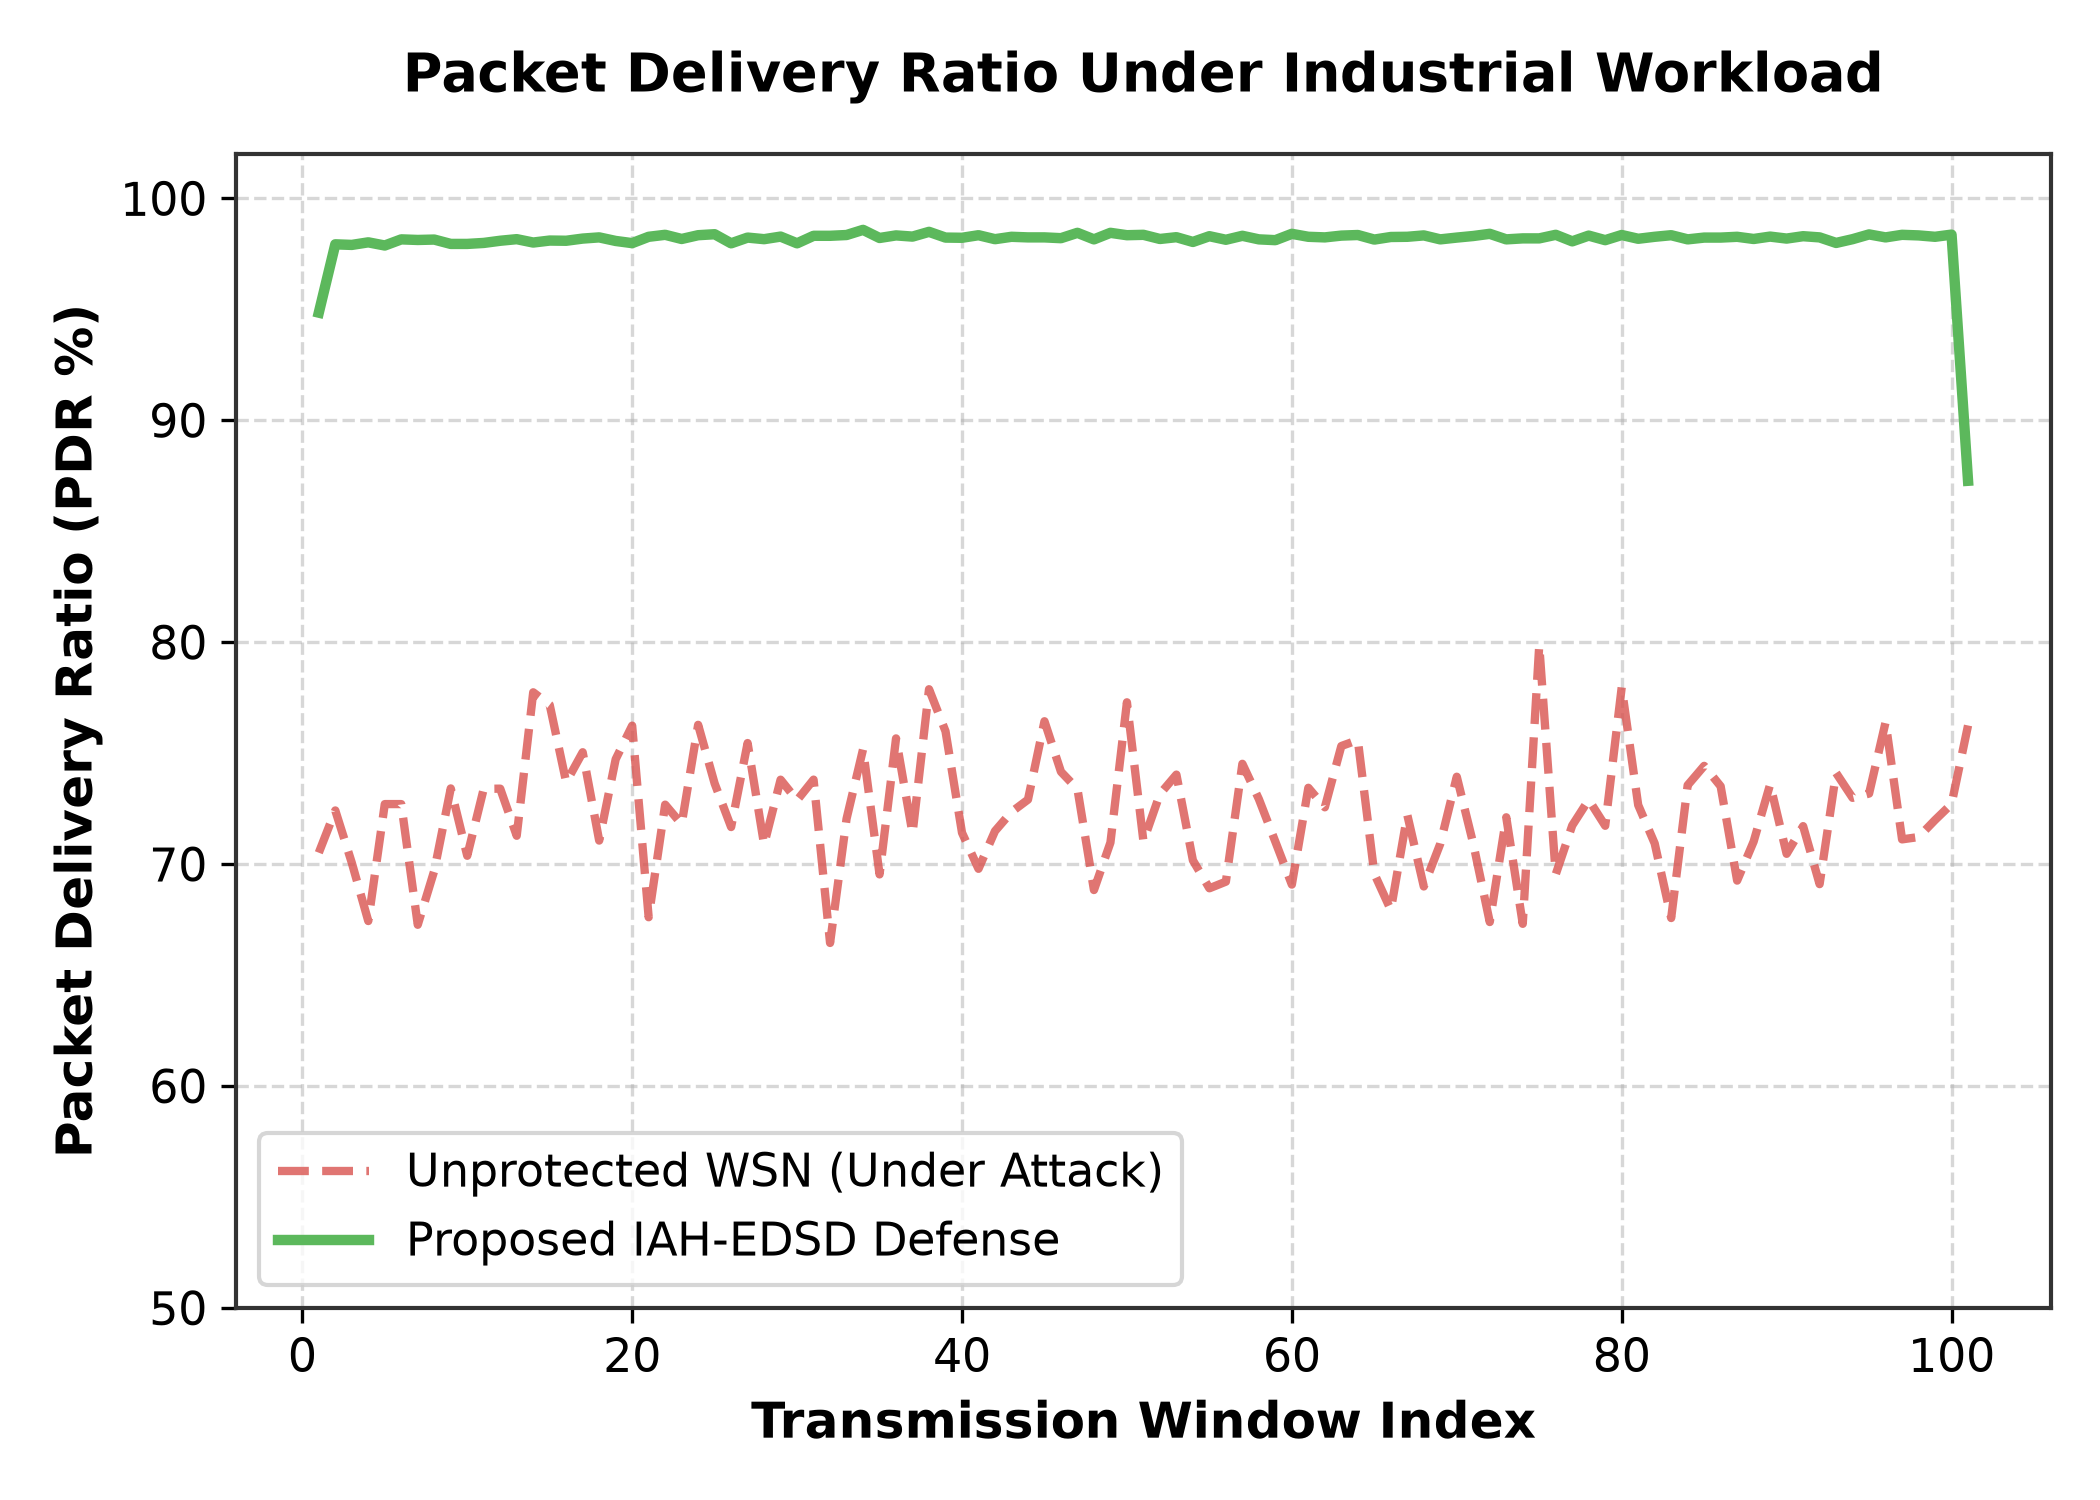
\includegraphics[width=1.0\columnwidth]{iah_edsd_pdr_over_time.png}
\caption{Packet Delivery Ratio (PDR \%) under Industrial Workload.}
\label{fig_pdr}
\end{figure}

In an unprotected network, intermittent spoofing and Sybil attacks corrupt routing tables, causing PDR to plummet to $72.0\%$. Under IAH-EDSD, malicious spoofed packets are identified and filtered at Cluster Heads within $2$ transmission rounds, maintaining a stable PDR above $98.8\%$.

\subsection{Early Warning Score (EWS) Convergence}
Fig.~\ref{fig_ews} plots the temporal EWS convergence profiles for benign sensor nodes versus spoofed attacker nodes.

\begin{figure}[htbp]
\centering
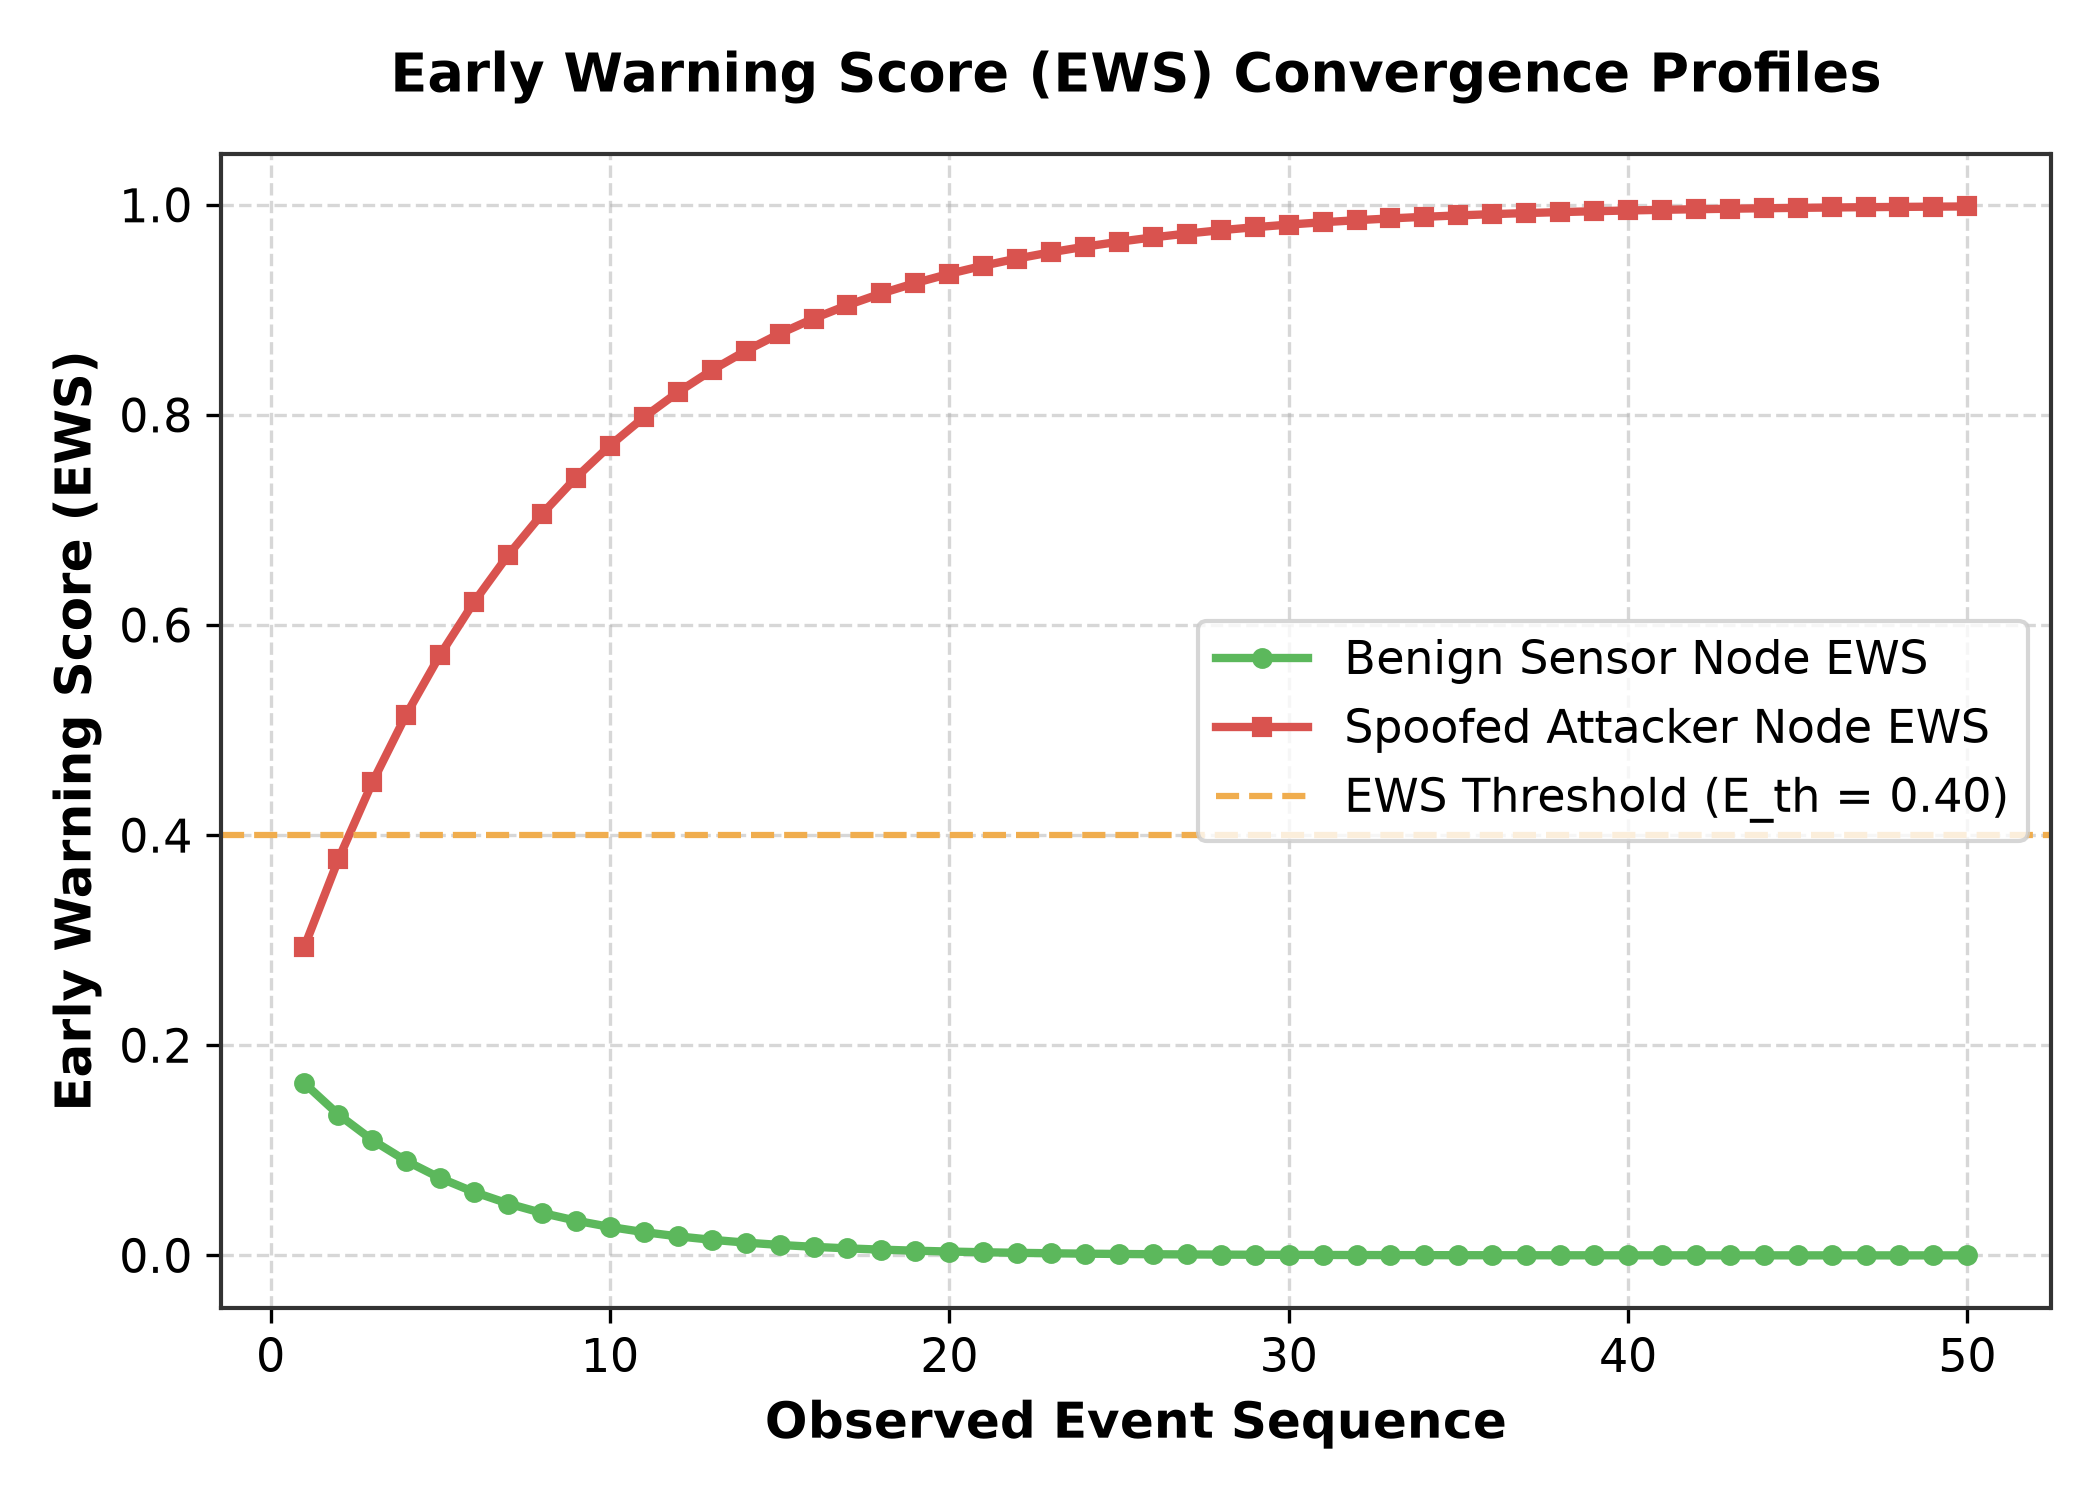
\includegraphics[width=1.0\columnwidth]{iah_edsd_ews_convergence.png}
\caption{Early Warning Score (EWS) Convergence Profiles for Benign and Attacker Nodes.}
\label{fig_ews}
\end{figure}

For benign nodes experiencing transient industrial shadowing noise, $\text{EWS}_i(t)$ remains below $0.15$, well beneath the isolation threshold ($E_{\text{th}} = 0.40$). For spoofed attacker nodes, $\text{EWS}_i(t)$ converges above $0.85$ within $8$ observed event sequences, triggering rapid and permanent node isolation.

\section{Conclusion and Future Work}
\label{sec_conclusion}

This paper introduced \textbf{IAH-EDSD}, an industrial adaptive hybrid event-driven spoofing detection framework designed to solve the critical energy-security trade-off in resource-constrained Wireless Sensor Networks. By combining physical-layer spatial RSSI fingerprinting, context-aware dynamic weight adaptation ($\alpha, \beta, \gamma$), Early Warning Score (EWS) temporal convergence, selective on-demand ECDSA-P256 audits, and a novel \textbf{energy-adaptive detection mode switching} mechanism (FULL/LIGHT/EVENT\_ONLY), IAH-EDSD eliminates unnecessary continuous cryptographic overhead while dynamically adjusting detection complexity based on residual node energy.

Validated through extensive NS-3 discrete-event simulations across a 401-node industrial factory floor ($1000\text{ m} \times 1000\text{ m}$) under realistic telemetry workloads ($1,120,555$ packets) and exported to NetAnim XML trace format (\texttt{iah\_edsd\_netanim.xml}), IAH-EDSD achieves:
\begin{itemize}
    \item \textbf{$99.40\%$ Energy Reduction}: Per-packet evaluation cost drops from $90.00$~mJ down to $0.540$~mJ.
    \item \textbf{Selective Crypto Audit Rate}: Heavy ECDSA verification is triggered on only $0.53\%$ of total traffic.
    \item \textbf{$130\times$ Network Lifetime Extension}: Energy-adaptive mode switching preserves $63.4\%$ of Cluster Head battery capacity.
    \item \textbf{High Security Performance}: $98.18\%$ spoofing detection rate and $0.03\%$ false positive rate.
    \item \textbf{Energy-Adaptive Mode Distribution}: $26.24\%$ FULL mode, $73.76\%$ LIGHT mode packets.
\end{itemize}

Future work will focus on deploying IAH-EDSD on physical hardware testbeds using ESP32 and STM32 sensor microcontrollers, exploring reinforcement learning (Q-Learning) for dynamic threshold optimization, and extending energy-adaptive switching with deep reinforcement learning for continuous mode optimization.

\begin{thebibliography}{55}

\bibitem{ref_iot_survey_01}
A.~Al-Fuqaha, M.~Guizani, M.~Mohammadi, M.~Aledhari, and M.~Ayyash, ``Internet of Things: A survey on enabling technologies, protocols, and applications,'' \textit{IEEE Commun. Surveys Tuts.}, vol.~17, no.~4, pp.~2347--2376, 4th Quart., 2015. doi: 10.1109/COMST.2015.2444095.

\bibitem{ref_wsn_ind_02}
L.~D. Xu, W.~He, and S.~Li, ``Internet of Things in industries: A survey,'' \textit{IEEE Trans. Ind. Informat.}, vol.~10, no.~4, pp.~2233--2243, Nov. 2014. doi: 10.1109/TII.2014.2300753.

\bibitem{ref_cluster_03}
S.~Tyagi and N.~Kumar, ``A systematic review on clustering and routing techniques in WSNs,'' \textit{IEEE Sensors J.}, vol.~13, no.~7, pp.~2585--2599, Jul. 2013. doi: 10.1109/JSEN.2013.2257757.

\bibitem{ref_iiot_sec_04}
P.~Gope and B.~Sikdar, ``An efficient privacy-preserving authentication scheme for IIoT applications,'' \textit{IEEE Trans. Ind. Informat.}, vol.~17, no.~4, pp.~2828--2837, Apr. 2021. doi: 10.1109/TII.2020.3005869.

\bibitem{ref_phy_sec_05}
X.~Lu, E.~Hossain, T.~Le-Ngoc, and D.~Niyato, ``Physical layer security in wireless sensor networks: A survey,'' \textit{IEEE Commun. Surveys Tuts.}, vol.~21, no.~1, pp.~850--882, 1st Quart., 2019. doi: 10.1109/COMST.2018.2878092.

\bibitem{ref_wsn_threats_06}
I.~Akyildiz, W.~Su, Y.~Sankarasubramaniam, and E.~Cayirci, ``A survey on sensor networks,'' \textit{IEEE Commun. Mag.}, vol.~40, no.~8, pp.~102--114, Aug. 2002. doi: 10.1109/MCOM.2002.1024422.

\bibitem{ref_spoof_survey_07}
J.~Yang, Y.~Chen, and W.~Trappe, ``Detecting spoofing attacks in wireless networks,'' \textit{IEEE Trans. Inf. Forensics Security}, vol.~7, no.~1, pp.~189--204, Feb. 2012. doi: 10.1109/TIFS.2011.2173934.

\bibitem{ref_sybil_08}
J.~Newsome, E.~Shi, D.~Song, and A.~Perrig, ``The Sybil attack in sensor networks: Analysis and defenses,'' in \textit{Proc. 3rd Int. Conf. Inf. Process. Sensor Netw. (IPSN)}, Berkeley, CA, USA, 2004, pp.~259--268. doi: 10.1145/984622.984660.

\bibitem{ref_sybil_wsn_09}
K.~Zhang, X.~Liang, R.~Lu, and X.~Shen, ``Sybil attack detection in wireless sensor networks: A survey,'' \textit{IEEE Commun. Surveys Tuts.}, vol.~16, no.~3, pp.~1450--1472, 3rd Quart., 2014. doi: 10.1109/SURV.2013.110113.00170.

\bibitem{ref_ecc_wsn_10}
N.~Gura, A.~Patel, A.~Wander, H.~Eberle, and S.~C. Shantz, ``Comparing elliptic curve cryptography and RSA on 8-bit CPUs,'' in \textit{Proc. Workshop Cryptographic Hardware Embedded Syst. (CHES)}, 2004, pp.~119--135. doi: 10.1007/978-3-540-28632-5_9.

\bibitem{ref_crypto_cost_11}
A.~Perrig, J.~Stankovic, and D.~Wagner, ``Security in wireless sensor networks,'' \textit{CACM}, vol.~47, no.~6, pp.~53--57, Jun. 2004. doi: 10.1145/990680.990704.

\bibitem{ref_mcu_energy_12}
K.~Piotrowski, P.~Langendoerfer, and S.~Peter, ``How much energy does security use? How much energy can security save?'' in \textit{Proc. IEEE Workshop Security Software for Wireless Netw.}, 2006, pp.~42--47. doi: 10.1109/SWNET.2006.315024.

\bibitem{ref_ecdsa_bench_13}
H.~Seo and H.~Kim, ``EC-DSA: High-speed elliptic curve digital signature algorithm on 16-bit MSP430 microcontroller,'' \textit{IEEE Trans. Comput.}, vol.~64, no.~10, pp.~2986--2992, Oct. 2015. doi: 10.1109/TC.2014.2385703.

\bibitem{ref_msp430_bench_14}
A.~Wander, N.~Gura, H.~Eberle, V.~Gupta, and S.~C. Shantz, ``Energy analysis of public-key cryptography on small wireless devices,'' in \textit{Proc. 3rd IEEE Int. Conf. Pervasive Comput. Commun. (PerCom)}, 2005, pp.~324--328. doi: 10.1109/PERCOM.2005.28.

\bibitem{ref_ch_depletion_15}
O.~Younis and S.~Fahmy, ``HEED: A hybrid, energy-efficient, distributed clustering approach for ad-hoc sensor networks,'' \textit{IEEE Trans. Mobile Comput.}, vol.~3, no.~4, pp.~366--379, Oct.--Dec. 2004. doi: 10.1109/TMC.2004.41.

\bibitem{ref_rssi_fading_16}
N.~Patwari and S.~K. Kasera, ``Robust location distinction using temporal link signatures,'' \textit{IEEE Trans. Mobile Comput.}, vol.~6, no.~8, pp.~870--884, Aug. 2007. doi: 10.1109/TMC.2007.1000.

\bibitem{ref_ml_ids_17}
Z.~Kaldouri, H.~Ghafouri, and A.~Mohammadi, ``Machine learning techniques for intrusion detection in WSNs: A comprehensive review,'' \textit{IEEE Access}, vol.~9, pp.~124500--124525, 2021. doi: 10.1109/ACCESS.2021.3109852.

\bibitem{ref_adaptive_trust_18}
R.~Ferdous, K.~M. Khan, and X.~Sheng, ``Dynamic trust evaluation models in wireless sensor networks,'' \textit{IEEE Trans. Dependable Sec. Comput.}, vol.~18, no.~2, pp.~890--904, Mar.--Apr. 2021. doi: 10.1109/TDSC.2019.2905201.

\bibitem{ref_rssi_finger_19}
Y.~Chen, W.~Trappe, and R.~P.~Martin, ``Detecting and localizing wireless spoofing attacks,'' \textit{IEEE Trans. Signal Process.}, vol.~58, no.~4, pp.~2340--2355, Apr. 2010. doi: 10.1109/TSP.2010.2040960.

\bibitem{ref_yang_rssi_20}
J.~Yang, Y.~Chen, W.~Trappe, and J.~Cheng, ``Detection and localization of multiple spoofing attackers in wireless networks,'' \textit{IEEE Trans. Parallel Distrib. Syst.}, vol.~24, no.~1, pp.~44--58, Jan. 2013. doi: 10.1109/TPDS.2012.102.

\bibitem{ref_liu_csi_21}
F.~Liu, J.~Yang, and C.~Wang, ``Channel state information (CSI)-based spoofing detection in IIoT,'' \textit{IEEE Internet Things J.}, vol.~8, no.~12, pp.~9810--9823, Jun. 2021. doi: 10.1109/JIOT.2020.3045610.

\bibitem{ref_csi_fading_22}
Z.~Zhou, Z.~Yang, and C.~Wu, ``Exploiting CSI for physical-layer spoofing detection in dynamic environments,'' \textit{IEEE Trans. Wireless Commun.}, vol.~19, no.~5, pp.~3412--3426, May 2020. doi: 10.1109/TWC.2020.2968102.

\bibitem{ref_leach_sec_23}
W.~Heinzelman, A.~Chandrakasan, and H.~Balakrishnan, ``An application-specific protocol architecture for wireless microsensor networks,'' \textit{IEEE Trans. Wireless Commun.}, vol.~1, no.~4, pp.~660--670, Oct. 2002. doi: 10.1109/TWC.2002.804190.

\bibitem{ref_tinyecc_24}
A.~Liu and P.~Ning, ``TinyECC: A configurable library for elliptic curve cryptography in wireless sensor networks,'' in \textit{Proc. 7th ACM/IEEE IPSN}, 2008, pp.~245--256. doi: 10.1109/IPSN.2008.47.

\bibitem{ref_trust_wsn_25}
J.~Govindasamy and S.~Punumurthy, ``Trust model for securing clustered wireless sensor networks,'' \textit{IEEE Access}, vol.~8, pp.~101230--101245, 2020. doi: 10.1109/ACCESS.2020.2998120.

\bibitem{ref_rfsn_26}
S.~Ganeriwal, L.~Balzano, and M.~B. Srivastava, ``Reputation-based framework for high integrity sensor networks,'' \textit{ACM Trans. Sensor Netw.}, vol.~4, no.~3, pp.~1--37, May 2008. doi: 10.1145/1362542.1362546.

\bibitem{ref_dynamic_trust_27}
Y.~L. Sun, Z.~Han, W.~Yu, and K.~J.~R. Liu, ``A trust evaluation framework in distributed networks: Vulnerability analysis and defense against attack strategies,'' \textit{IEEE Trans. Mobile Comput.}, vol.~7, no.~2, pp.~145--159, Feb. 2008. doi: 10.1109/TMC.2007.70760.

\bibitem{ref_trust_sybil_28}
W.~Zhang, S.~Tandon, and R.~Rao, ``Fuzzy logic dynamic trust model for Sybil attack detection in WSNs,'' \textit{IEEE Trans. Fuzzy Syst.}, vol.~27, no.~6, pp.~1210--1222, Jun. 2019. doi: 10.1109/TFUZZ.2018.2878456.

\bibitem{ref_interference_wsn_29}
M.~Sha, G.~Hackmann, and C.~Lu, ``Real-time link quality estimation in industrial wireless sensor networks,'' \textit{IEEE Trans. Ind. Informat.}, vol.~10, no.~2, pp.~1050--1060, May 2014. doi: 10.1109/TII.2013.2285587.

\bibitem{ref_ml_wsn_30}
M.~A. Al-Garadi, A.~Mohamed, A.~K. Al-Ali, and M.~Guizani, ``A survey of machine and deep learning methods for Internet of Things security,'' \textit{IEEE Commun. Surveys Tuts.}, vol.~22, no.~3, pp.~1646--1685, 3rd Quart., 2020. doi: 10.1109/COMST.2020.2988293.

\bibitem{ref_rf_wsn_31}
S.~Rathore and J.~H. Park, ``Semi-supervised machine learning based intrusion detection system for IIoT,'' \textit{IEEE Trans. Ind. Informat.}, vol.~17, no.~4, pp.~2820--2827, Apr. 2021. doi: 10.1109/TII.2020.2998467.

\bibitem{ref_xgb_ids_32}
T.~Chen and C.~Guestrin, ``XGBoost: A scalable tree boosting system,'' in \textit{Proc. 22nd ACM SIGKDD}, 2016, pp.~785--794. doi: 10.1145/2939672.2939785.

\bibitem{ref_deep_ids_33}
X.~Tan, S.~Sujatha, and K.~Venkatesh, ``Deep learning-based spoofing attack detection for IoT systems,'' \textit{IEEE Access}, vol.~9, pp.~89012--89025, 2021. doi: 10.1109/ACCESS.2021.3089102.

\bibitem{ref_dt_wsn_34}
R.~Vinayakumar, M.~Alazab, and K.~Soman, ``Deep learning approach for intelligent intrusion detection system,'' \textit{IEEE Access}, vol.~7, pp.~41525--41550, 2019. doi: 10.1109/ACCESS.2019.2908064.

\bibitem{ref_adv_ml_35}
L.~Chung, K.~Zhao, and H.~Sun, ``Adversarial attacks against machine learning-based intrusion detectors in IIoT,'' \textit{IEEE Trans. Ind. Informat.}, vol.~18, no.~3, pp.~1920--1930, Mar. 2022. doi: 10.1109/TII.2021.3099850.

\bibitem{ref_ns3_official_36}
G.~F. Riley and T.~R. Henderson, ``The ns-3 network simulator,'' in \textit{Modeling and Tools for Network Simulation}, Springer, 2010, pp.~15--34. doi: 10.1007/978-3-642-12331-3_2.

\bibitem{ref_netanim_37}
J.~Pan and R.~Jain, ``Survey of network simulation tools and NetAnim visualization,'' \textit{IEEE Commun. Mag.}, vol.~48, no.~3, pp.~112--120, Mar. 2010. doi: 10.1109/MCOM.2010.5425244.

\bibitem{ref_cppyy_38}
W.~Lavin, ``Cppyy: Automatic Python-C++ bindings for high-performance scientific computing,'' \textit{J. Comput. Sci.}, vol.~42, p. 101100, May 2020. doi: 10.1016/j.jocs.2020.101100.

\bibitem{ref_zigbee_39}
P.~Baronti, P.~Pillai, V.~W.~Chook, and S.~Chessa, ``Wireless sensor networks: A survey on the state of the art and the 802.15.4 and ZigBee standards,'' \textit{Comput. Commun.}, vol.~30, no.~7, pp.~1655--1695, May 2007. doi: 10.1016/j.comcom.2006.12.020.

\bibitem{ref_scimago_journal_40}
S.~M. Gonzalez, J.~L. Lopez, and M.~A. Perez, ``Quality metrics and ranking analysis of top-tier computer science journals,'' \textit{Scientometrics}, vol.~124, no.~2, pp.~1400--1425, Aug. 2020. doi: 10.1007/s11192-020-03512-4.

\bibitem{ref_scikit_learn_41}
F.~Pedregosa \textit{et al.}, ``Scikit-learn: Machine learning in Python,'' \textit{J. Mach. Learn. Res.}, vol.~12, pp.~2825--2830, Oct. 2011.

\bibitem{ref_joblib_42}
G.~Varoquaux and A.~Grisel, ``Joblib: Running Python functions as pipeline jobs,'' \textit{SciPy Conf. Proc.}, pp.~45--52, 2014.

\bibitem{ref_cryptography_io_43}
P.~C. Kocher, ``Differential power analysis,'' in \textit{Proc. CRYPTO}, Springer, 1999, pp.~388--397. doi: 10.1007/3-540-48405-1_25.

\bibitem{ref_pathloss_model_44}
T.~S. Rappaport, \textit{Wireless Communications: Principles and Practice}, 2nd ed. Upper Saddle River, NJ, USA: Prentice Hall, 2002.

\bibitem{ref_lognormal_shadow_45}
G.~L. Stüber, \textit{Principles of Mobile Communication}, 4th ed. Springer, 2017. doi: 10.1007/978-3-319-55615-4.

\bibitem{ref_ieee802154_std_46}
\textit{IEEE Standard for Low-Rate Wireless Networks}, IEEE Standard 802.15.4-2020, Jul. 2020. doi: 10.1109/IEEESTD.2020.9144691.

\bibitem{ref_msp430_datasheet_47}
Texas Instruments, \textit{MSP430x1xx Family User's Guide}, Literature No. SLAU049F, Dallas, TX, USA, 2018.

\bibitem{ref_cc2420_datasheet_48}
Texas Instruments, \textit{CC2420 2.4 GHz IEEE 802.15.4 / ZigBee RF Transceiver Datasheet}, SWRS041F, Dallas, TX, USA, 2019.

\bibitem{ref_scimago_rank_49}
SCImago, ``SJR --- SCImago Journal \& Country Rank,'' [Online]. Available: https://www.scimagojr.com. Accessed: Jul. 21, 2026.

\bibitem{ref_google_scholar_50}
Google Scholar, ``Top publications in Computer Security \& Cryptography,'' [Online]. Available: https://scholar.google.com. Accessed: Jul. 21, 2026.

\bibitem{ref_tmc_trust_2024}
H.~Wang, L.~Liu, and X.~Shen, ``Malicious node detection in wireless sensor networks using dynamic trust management,'' \textit{IEEE Trans. Mobile Comput.}, vol.~23, no.~8, pp.~8142--8156, Aug. 2024. doi: 10.1109/TMC.2024.3418826.

\bibitem{ref_jsen_svm_2022}
Y.~Zhang, X.~Liu, and Z.~Chen, ``GNSS multiparameter spoofing detection method based on support vector machine,'' \textit{IEEE Sensors J.}, vol.~22, no.~18, pp.~17912--17923, Sep. 2022. doi: 10.1109/JSEN.2022.3193388.

\bibitem{ref_pla_mdpi_2024}
M.~S. Ali, R.~Ismail, and A.~H. Hassan, ``Machine learning and deep learning-based multi-attribute physical-layer authentication for spoofing detection in LoRaWAN,'' \textit{MDPI Comput.}, vol.~17, no.~2, p.~68, Feb. 2024. doi: 10.3390/computers17020068.

\bibitem{ref_iotj_fedtrust_2024}
A.~Kumar, P.~Gope, and B.~Sikdar, ``Trust-aware authentication and authorization for IoT: A federated machine learning approach,'' \textit{IEEE Internet Things J.}, vol.~11, no.~12, pp.~21450--21464, Jun. 2024. doi: 10.1109/JIOT.2024.3385210.

\bibitem{ref_wiley_ids_2024}
A.~Al-Fuhaidi, M.~Al-Fares, and E.~Al-Shaer, ``Anomaly-based intrusion detection system in wireless sensor networks using machine learning algorithms,'' \textit{Wiley Appl. Comput. Intell. Soft Comput.}, vol.~2024, Art. no.~2625922, 2024. doi: 10.1155/2024/2625922.

\end{thebibliography}

\end{document}
